\documentclass[11pt,a4paper,twoside]{thesis}

\usepackage{graphicx}
\usepackage[utf8]{inputenc}
\usepackage[spanish]{babel}
\usepackage[left=3cm,right=3cm,bottom=3.5cm,top=3.5cm]{geometry}
\usepackage{titlesec}
\usepackage{listings}
\usepackage{xcolor}
\usepackage{hyperref}
\usepackage{amsmath}
\usepackage{amssymb}
\usepackage[utf8]{inputenc}
\usepackage{enumitem}
\usepackage{booktabs}

\begin{document}

%%%% CARATULA

\def\autor{Adrian Norberto Marino}
\def\tituloTesis{Sistemas de Recomendación Colaborativos}
\def\runtitulo{Resumen}
\def\runtitle{Sistemas de Recomendación Colaborativos}

%\def\director{Obi-Wan Kenobi}
%\def\codirector{Master Yoda}

\def\lugar{Buenos Aires, 2022}

% -----------------------------------------------------------------------------
% Caratula,  Resumen, agradecimientos y dedicatoria.
% -----------------------------------------------------------------------------
\newcommand{\HRule}{\rule{\linewidth}{0.2mm}}
%
\thispagestyle{empty}

\begin{center}\leavevmode

	\vspace{-2cm}

	\begin{tabular}{l}
		
\includegraphics[width=4.6cm]{./images/logouba.png}
	\end{tabular}

	{\large \sc Universidad de Buenos Aires\\Facultad de Ciencias Exactas y Naturales \\ Facultad de Ingeniería}

	\vspace{5.0cm}

	\begin{huge}
		\textbf{\tituloTesis}
	\end{huge}

	\vspace{2cm}

	{\large Traba de tesis de la \textit{Maestría en Explotación de Datos y Descubrimiento del Conocimiento}}
	\vspace{2cm}

	{\large \href{https://github.com/adrianmarino/thesis-paper}{Proyecto en Gihub}}

	\vspace{2cm}

	{\Large \autor}

\end{center}

\vfill

{\large

	{Director: \director}

	\vspace{.2cm}

	\lugar
}

\newpage\thispagestyle{empty}

%
\frontmatter
\pagestyle{empty}
%\begin{center}
%\large \bf \runtitulo
%\end{center}
%\vspace{1cm}
\chapter*{\runtitulo}

\noindent Este trabajo de tesis experimenta con el uso de grandes modelos de lenguaje (\textit{Large language Models o LLM}) como interfaz de comunicación con el usuario final. Estos modelos se emplean para la búsqueda de contenido personalizado para el usuario en respuesta a consultas en lenguaje natural. El sistema de recomendaciones es capaz de ofrecer contenido personalizado al usuario y aborda el problema del \textit{Cold start} mediante un \textit{ensamble} de modelos de recomendación basados en contenido, filtros colaborativos y modelos de lenguaje.

\bigskip

\noindent\textbf{Palabras claves:} \textit{LLM}, \textit{Cold Start}, Sistemas de recomendación basados en Filtro Colaborativos, Sistemas de recomendación en basados en contenido, \textit{API}, \textit{RAG}, \textit{ChromaDB}, \textit{Apache Airflow}, \textit{Llama}, Máquinas de factorización profundas (\textit{DeepFM}).
%
%\cleardoublepage
%\chapter*{Agradecimientos}

\noindent  % OPCIONAL: comentar si no se quiere
%
\cleardoublepage
\chapter*{Agradecimientos}

\hfill \textit{Principalmente a mis padres, siempre fueron un gran apoyo en mi carrera, alentándome incansablemente para seguir adelante en todo momento. Gran parte de mi disciplina de constante persistencia se la debo a ellos. En segundo lugar a mis profesores de la especialización y maestría, por entregarnos su conocimiento dia a dia, siempre enfocados en que comprendamos todos los temas expuesto de la mejor forma posible. A mis compañeros de la especialización, siempre fueron un gran grupo de apoyo, un grupo en el que nos ayudamos uno al otro para comprender los temas expuestos.}
  % OPCIONAL: comentar si no se quiere
% -----------------------------------------------------------------------------
%
%
%
%\cleardoublepage
\tableofcontents
%
%
\mainmatter
\pagestyle{headings}
%
%
%
%
% -----------------------------------------------------------------------------
% Contenido de la tesis
% -----------------------------------------------------------------------------

\setitemize{itemsep=0.5pt}

\chapter{Introducción}

Los sistemas de recomendación tienen como objetivo principal proporcionar a los
usuarios productos, promociones y contenidos relevantes a sus preferencias o
necesidades. Estos sistemas permiten a los usuarios encontrar de forma ágil y
eficiente lo que están buscando. Formalizando esta definición, podemos decir
que los sistemas de recomendación buscan ayudar a un usuario o grupo de
usuarios a descubrir ítems que se ajusten a sus preferencias, dado un conjunto
de ítems que puede ser extenso o un amplio espacio de búsqueda.

\begin{sloppypar}
	Este objetivo puede variar dependiendo de cada negocio: Si consideramos un
	\textit{e-commerce} de \textit{delivery} gastronómico, su propósito sería
	ofrecer a los clientes platos relevantes a un precio asequible y con un tiempo
	de entrega aceptable.
\end{sloppypar}

Si hablamos de un \textit{e-commerce} de productos, su objetivo consiste en
proporcionar a los usuarios aquellos productos que satisfacen sus necesidades, a
un precio que estén dispuestos a pagar. Además, se busca garantizar una
experiencia satisfactoria con los vendedores.

En el negocio de visualización de contenido (audio, video, texto, etc..), el
objetivo es acercar a sus usuarios contenido a fin a sus preferencias para
mejorar su experiencia en la plataforma.

El objetivo principal en todos los casos es mejorar la conversión. En el campo
del \textit{marketing}, se define la conversión como las acciones realizadas
por los usuarios que están alineadas con los objetivos de la empresa. Por
ejemplo, aumentar el volumen de compras en un \textit{e-commerce} de productos,
incrementar la cantidad de entregas mensuales en un \textit{e-commerce} de
\textit{delivery} gastronómico, aumentar las impresiones de publicidad en
aplicaciones de visualización de contenido, prolongar el tiempo de permanencia
en plataformas de \textit{streaming} de audio o video, entre otros. Existen
numerosos ejemplos en los que el objetivo común es mejorar la conversión y el
compromiso del usuario con la marca, es decir, el \textit{engagement}.

Desde un enfoque técnico, los sistemas de recomendación se utilizan para
predecir el grado de preferencia de un usuario con un artículo específico. Esto
se logra aplicando algoritmos de optimización que minimizan la diferencia entre
el grado de preferencia esperado y el grado de preferencia real del usuario.
También existen otros enfoques que utilizan medidas de distancia para
determinar este grado de preferencia. En secciones posteriores, exploraremos
estos conceptos con mayor detalle.

\clearpage
\section{Tipos de sistemas de recomendación}

A continuación, en la figura~\ref{fig:clasification}, se pueden observar las
diferentes categorías y sub-categorías de los sistemas de recomendación:

\begin{figure}[!htb]
	\centering
	\includegraphics[width=12cm]{./images/clasificacion-sis-rec.png}
	\caption{Clasificación de tipos de sistemas de recomendaciones.}
	\label{fig:clasification}
\end{figure}

\subsection{Basados en Popularidad}

Este tipo de sistema de recomendación utiliza alguna característica de
popularidad de los ítems en cuestión. Algunos ejemplos de estas características
podría ser la cantidad de vistas, la cantidad de compras o la cantidad de
comentarios positivos, o una combinación de ellas. Luego, estos sistemas buscan
los K elementos más populares. Si bien este tipo de enfoque proporciona buenos
resultados para nuevos usuarios, sus recomendaciones no tienen en cuenta las
preferencias individuales de cada usuario, ya que se basan en estadísticas
comunes a todos los usuarios. Por esta razón, a menudo no se consideran
sistemas de recomendación en sentido estricto. No obstante, siguen siendo
ampliamente utilizados debido a su capacidad para generar una alta tasa de
conversión, a pesar de la falta de personalización.

\subsection{Basados en Contenido}

Este tipo de sistema de recomendación necesita un trabajo previo de ingeniería
de \textit{features} sobre los ítems. Se busca definir cuales son los
\textit{features} mas significativos para la tarea en cuestión, y cual es el
grado de adecuación de cada ítems a los \textit{features} seleccionados. Por
otro lado, es necesario registrar las interacciones de los usuarios. Dadas
estas interacciones, se puede definir el grado de preferencia de los usuarios a
cada \textit{feature} definido para los ítems. Con esta información, es posible
encontrar tanto ítems como usuarios similares y realizar recomendaciones del
tipo:

\begin{itemize}
	\item Dado el \textit{Usuario A}, el cual tiene preferencia por el \textit{Ítem X},
	      también podría tener preferencia por el \textit{Ítem Y}, por ser muy cercano o
	      similar al \textit{Ítem X}.
	\item Dos \textit{Usuarios A y B} cercanos o similares, tendrán preferencias
	      similares. De esta forma es posible recomendar ítem consumidos por el
	      \textit{Usuario A} al \textit{Usuario B} y vise versa.
\end{itemize}

La principal desventaja de este enfoque, es la necesidad de realizar ingeniería
de \textit{features} para encontrar los \textit{features} que produzcan
recomendaciones relevantes al usuario. El modelo no encuentra estos
\textit{features} automáticamente, sino que deben ser definidos de antemano
manualmente. Se puede apreciar que esto introduce un sesgo al momento de
seleccionar los \textit{features} o construirlos en base a datos referentes a
los ítems. Como ventaja, si se encuentran los \textit{features} correctos se
pueden lograr muy buenos resultados.

\subsection{Basados en Filtrado Colaborativos}

Estos modelos, a diferencia de los modelos basados en contenido, no requirieren
ingeniería de \textit{features}, lo que hace muy simple su implementación, ya
que únicamente es necesario registrar las interacciones de los usuarios para
con los ítems. Luego, el propio modelo encuentra automáticamente los
\textit{features} mas relevantes dependiendo de la cantidad de columnas que se
especifiquen (dimensiones de un vector \textit{Embedding}). Ejemplos de
interacciones podrían ser:

\begin{itemize}
	\item El \textit{Usuario A} visualizo el \textit{Ítem X} el dia 2 de marzo de 2022.
	\item El \textit{Usuario A} compro el \textit{Ítem X} el dia 10 de marzo de 2022.
	\item El \textit{Usuario A} califico al \textit{Ítem X} con 5 puntos el dia 25 de
	      marzo de 2022.
\end{itemize}

Ambos tipo de modelos, basados en contenido y filtros colaborativos,
personalizan sus recomendaciones. Es decir, ajustan las recomendaciones a las
preferencias de cada usuario particular. Además, ambos permiten encontrar
usuarios e ítems similares y recomendar ítems entre usuarios similares.

Por otro lado, los modelos basados en filtros colaborativos, descubren un
espacio latente de soluciones sin necesidad de recolectar datos y definir
\textit{features} en forma manual, a diferencia de los modelos basados en
contenido. La selección o construcción manual de \textit{features} puede llevar
a una solución sesgada, ya que no esta basada en datos sino en el juicio
experto del científico de datos. Esto puede llevar a una selección subjetiva de
los \textit{features} que se aleje de la realidad, introduciendo un sesgo en la
predicción.

No todo son rosas con estos modelos, dado que sufren un problema llamado
\textit{Cold start} o arranque en frio. Los usuarios nuevos son aquellos que
aun no han realizado ninguna interacción con el sistema. Estos modelos no
podrán realizar recomendaciones a estos usuarios, dado que requieren un mínimo
de interacciones para comenzar a ofrecer recomendaciones con cierta precisión.

Además, existen otros problemas referidos al cambiar la cantidad de
interacciones de los usuarios. Si pensamos en una solución donde alimentamos al
modelo con una ventana de interacciones para los últimos N meses, tendremos las
siguiente situaciones:

\begin{itemize}
	\item Usuarios nuevos: Los usuarios nuevos no tendrán interacciones. Por lo tanto,
	      este modelo no podrá realizar ninguna recomendación. En general, se establece
	      un mínimo de interacciones para que el modelo pueda realizar recomendaciones de
	      forma acertada.
	\item Usuarios con pocas interacciones: Por otro lado, tenemos a los usuarios que
	      tienen una baja taza de interacciones con el sistema o aplicación. Por ejemplo,
	      en un \textit{e-commerce} de venta de productos, hay usuarios que compran con
	      mucha frecuencia y otros muy de vez en cuando. Estos últimos, en general
	      tendrán una baja taza de interacción pudiendo caer por debajo del umbral mínimo
	      que requiere el modelo. De esta forma, tendremos usuarios que quedarán fuera
	      del modelo actual.
	\item Usuarios con muchas interacciones: En este caso, el usuario tiene una gran
	      cantidad de interacciones con ítems. Para estos usuarios, el modelo podrá
	      ofrecer recomendaciones relevantes, ya que cuanto mas interacciones se tenga,
	      el modelo se ajusta con mas facilidad a sus preferencias. Por otro lado, esto
	      puede ser una gran desventaja, ya que se produce un efecto de túnel. Es decir,
	      el usuario obtiene recomendaciones muy ajustadas a sus preferencias, perdiendo
	      la capacidad de descubrir nuevos ítems que podrían ser relevantes. Por esta
	      cuestión se suelen mezclar tanto recomendaciones personalizadas como
	      no-personalizadas, para favorecer el descubrimiento de nuevos ítems.

\end{itemize}

\clearpage
\subsection{Modelos Híbridos}

Son aquellos modelos que combinan mas de una técnica de recomendación, también
llamados ensambles de modelos. Comúnmente están compuestos por modelos de
recomendación por popularidad, basados en contenido y filtros colaborativos. De
esta forma, cuando los usuarios caen por debajo del umbral de interacciones
necesarias por el modelo de filtro colaborativos, se utiliza un modelos basado
en contenido, popularidad, o algún otro modelo que no requiere de interacciones
del usuario para realizar sus recomendaciones.

\subsection{Categorías dentro de los modelos basados en filtros colaborativos}

Dentro de los sistemas de recomendación basados en filtros colaborativos,
tenemos dos sub-clasificaciones referidas a la forma en la que se realizan las
predicciones.

\subsubsection{Basados en Memoria}

Este tipo de modelos, como su nombre lo indica, mantiene sus datos en memoria.
Se recorren todos los datos (\textit{full scan}) cada vez que se necesita
realizar un inferencia o predicción (fijando un número de vecinos a comparar).
Un ejemplo de estos modelos es el algoritmo de k vecinos cercanos
(\textit{KNN}), el cual mantiene una matriz rala de distancias en memoria, la
cual se recorre completamente para comparar las distancias entre filas o
columnas, usando alguna medida de distancia como puede ser la \textit{distancia
	coseno}, \textit{coseno ajustada}, \textit{manhattan}, etc.. Para mitigar el
problema de búsqueda exhaustiva (\textit{full scan}), se puede utilizar una
memoria \textit{cache} y asi realizar estas búsquedas una única vez. Otro
problema es su limitación al tamaño máximo de la memoria con la que se cuenta,
es decir, que el tamaño de la matriz depende de la memoria máxima disponible.
Esto puede mitigarse utilizando implementaciones de matrices rala, las cuales
comprimen los datos en memoria guardando unicamente las celdas que tienen
datos. Además, es posible utilizar un memoria \textit{cache} que mantenga en
memoria las búsqueda mas frecuentes y baje a almacenamiento secundario las
menos frecuentes. Todos estos problemas de \textit{performance} y uso de
recursos se deben a que \textit{KNN} no reduce la dimensionalidad de los datos,
como si lo hacen varias implementaciones basadas en \textit{embeddings},
\textit{auto-encoder}, redes neuronales etc.., donde lo que se busca una
representación mas compacta de los ítems y usuarios sin perder información. Mas
allá de estos problemas, los resultados obtenidos por estos modelos no están
muy alejados de aquellos que se encuentran en el estado del arte. Puede
recomendarse su uso cuando tenemos un dominio reducido, dada su simplicidad.

\subsubsection{Basados en Modelos}

Algunos ejemplos de estos modelos son los clasificadores bayesianos, redes
neuronales, algoritmos genéticos, sistemas difusos y la técnica de
descomposición matricial (\textit{SVD}). Estos modelos en general buscan
directa o indirectamente reducir la dimensionalidad de los datos. De esta
forma, es posible utilizarlos en dominios con una gran cantidad de datos.

\clearpage
\section{Descripción del problema y motivación}

Con este trabajo se busca contestar a las siguientes preguntas:

\subsection{¿Los modelos basado en filtro colaborativos que utilizan técnicos de \textit{Deep Learning}, obtienen mejores resultados que aquellas que no las utilizan?}

La idea detrás de esta pregunta es realizar \textit{benchmarks} sobre distintos
modelos del estado de arte basados en \textit{Deep Learning} o no, utilizando
el mismo set de datos y las mismas métricas. De esta forma, se busca comprender
cual es la diferencia en \textit{performance} entre los modelos seleccionados.
Por otro lado, se busca comprender cuando es mas adecuado utilizar cada
enfoque. Como ya se comentó en el apartado de introducción, hay modelos que
están mas limitados que otros según el número de recursos de \textit{hardware}
o interacciones con los que se cuenta.

\subsection{¿Cuáles son las ventajas y desventajas de cada enfoque a la hora de aplicar estas técnicas?}

Esta pregunta se refiere a comprender cuando es conveniente aplicar una técnica
u otra teniendo en cuenta las ventajas y desventajas de cada enfoque y modelo.

\subsection{¿Cómo se puede solucionar el problema de \textit{Cold start}
	que sufre el enfoque de recomendación basado en filtros colaborativos? (tesis)}

Como ya se comentó en la introducción, los modelos de filtro colaborativos
necesitan un número mínimo de interacciones usuario-ítem para poder operar y
producir recomendaciones aceptables. La propuesta es explorar enfoques que
permiten lidiar con este problema. Uno de los enfoques más comunes es utilizar
ensambles de modelos basados en filtros colaborativos con otros modelo basados
en contenidos o popularidad. Estos ensambles puede diferir en sus técnicas
dependiendo del dominio de los datos.

\section{Objetivos}

Como primer objetivo, se pretender comprender cuales son los fundamentos
teóricos sobre los que se apoya cada técnica aplicada y bajo que escenarios
puede ser conveniente aplicarlas. Por otro lado, se intenta determinar cual es
la diferencia en \textit{performance} de cada técnica aplicada sobre el mismo
set de datos, midiendo su \textit{performance} utilizando las mismas métricas.
¿Obtenemos diferencias significativas?

Como segundo objetivo (tesis), se busca proponer nuevas técnicas y/o explorar
técnicas existentes que permite lidiar o solucionar el problema de \textit{Cold
	start} que sufren los sistemas de recomendación basados en filtros
colaborativos. Ademas, se compararan esta técnicas mediante un
\textit{benchmark} propuesto, para compara como se comporta cada modelos ante
usuarios con escasas o ninguna interacción en el set de datos propuesto.

\chapter{Materiales y Métodos}

\section{Datos}


\chapter{Métodos}

En este capitulo se describirán los modelos utilizados para realiza la
predicción de la clasificación de un usuario para una película que aun no ha
visto. Para realizar esto, se utilizaron varios modelos basados en filtros
colaborativos.

Cada implementación tiene sus particularidades: Su nivel de escalabilidad, sus
tiempos de entrenamiento y predicción, su implementación, la exactitud de las
predicciones, su tendencia al sobre ajuste, etc.. Para este trabajo se
eligieron dos grandes grupos. Por un lado, una implementación sencilla basada
en memoria, como es el algoritmo de K vecinos cercanos. Por otro lado, modelos
basados en \textit{Deep Learning}. Los modelos basados en \textit{Deep
	Learning} utilizan \textit{Embeddings} en todos los casos, como una forma de
reducir la dimensionalidad de las variables categóricas que se utilizan como
entradas al modelo. Además, cada modelo tiene su propia arquitectura, algunas
clásicas y otras basadas en modelos del estado del arte. Luego, la idea fue
medir los resultados de todo los modelos, utilizando distintas métricas
comparables, entrenando con el mismo \textit{dataset} en todos los casos. De
esta forma podemos comparar los resultados de todos los modelos. Como
\textit{baseline} se tomo el modelo de K vecinos cercanos (\textit{KNN}), dado
que es el modelo mas simple. Este servirá como punto partida para comparar
resultados con otros modelos mas complejos.

Por otro lado, dada la cantidad de datos con la que se cuenta y teniendo en
cuenta que estos modelos son muy demandantes en cuanto a recursos de
\textit{hardware}, se opto por usar el framework
\href{https://pytorch.org/}{\textit{PyTorch}}. Dado que permite hacer uso tanto
de \textit{CPU} como \textit{GPU}. De esta forma, se puede elegir cuando usar
cada dispositivo y en que parte del flujo (pre-procesamiento, entrenamiento e
inferencia). Ya elegido el \textit{framework}, se opto por implementar todos
los modelos desde sus bases, ya que \textit{PyTorch} no cuenta con mucho
modelos del estado del arte desarrollados de forma oficial. De esta forma se
implemento cada modelo desde cero para poder hacer uso de \textit{CPU} y
\textit{GPU} de forma granular y realizar un uso mas eficiente de los recursos
disponible. Mas adelante veremos que esto puede impactar fuertemente en los
tiempos de entrenamiento e inferencia.

\clearpage

\section{Enfoque Basados en Memoria}

\subsection{
	Algoritmo de los K vecinos cercanos (\textit{K-Nearest-Neighbor}
	o \textit{KNN}) }

Esta es la implementación clásica y mas intuitiva para realizar recomendación
de ítems. Una vez entrenado el modelo, se cuenta con una matriz de distancias
que pueden ser: distancias entre usuarios o ítems, y otra matriz de
calificaciones usuario-ítem. De esta forma, en la etapa de inferencia, el
modelo toma como entrada un usuario (\textit{user\_id}) y un ítem
(\textit{item\_id}) y retorna la predicción de la calificación. Estas matrices
se puede mantener en memoria, persistir en una base de datos (como puede ser
\textit{Redis}) o en un archivos indexado. Por esta cuestión, la categoría en
memoria no tiene por que ser estricta, pero si se entiende que los mejores
tiempos de inferencia y entrenamiento se lograran cuando se tenga parte o la
totalidad de estas matrices en memoria.

Luego, para realizar el entrenamiento del modelo se necesita una lista de
tuplas, donde cada tupla contiene:

\begin{description}
	\item[Lista de tuplas]
\end{description}
\begin{equation}
	Tuplas = [<u_1; i_1; r_{u_1, i_1}>,...,<u_n; i_m; r_{u_n, i_m}>]
\end{equation}
\begin{description}
	\item[Donde:]
\end{description}
\begin{itemize}
	\item $u$ es un identificador secuencial, univoco y numérico de un usuario. Estos identificadores se generan a partir de una secuencia numérica, es decir que no debemos tener huecos para minimizar el uso de memoria en caso de no usar matrices ralas.
	\item $i$ es un identificador secuencial, univoco y numérico de un ítem. En este caso los ítems son películas, pero podrían ser cualquier entidad identificable como productos, usuarios, comidas, etc..
	\item $r_{u, i}$ es la calificación otorgada al ítem $i$ por parte del usuario $u$.
	\item $n$ es la cantidad total de usuarios en el \textit{dataset} de entrenamiento.
	\item $m$ es la cantidad total de ítems en el \textit{dataset} de entrenamiento.
\end{itemize}

Dada esta lista de tuplas, podemos construir una matriz esparza donde cada fila
representa a un usuario y cada columna a un ítem o vise versa, y las celdas o
valores de la misma contienen las calificaciones.

\begin{description}
	\item[Matriz de calificaciones]
\end{description}
\begin{equation}
	Calificaciones_{u,i} =
	\begin{pmatrix}
		r_{1,1} & r_{1,2} & \cdots & r_{1,i} \\
		r_{2,1} & r_{2,2} & \cdots & r_{2,i} \\
		\vdots  & \vdots  & \ddots & \vdots  \\
		r_{u,1} & r_{u,2} & \cdots & r_{u,i}
	\end{pmatrix}
\end{equation}

\clearpage

\begin{description}
	\item[Donde:]
\end{description}
\begin{itemize}
	\item $r_{u,i}$ es la calificación otorgada al ítem $i$ por parte del usuario $u$.
	\item Cada vector fila $F_u$ contiene todas la calificaciones realizadas por el
	      usuario $u$ para todos los ítems. Los ítems que aun no tiene calificación
	      contiene el valor $0$.
	\item Cada vector columna $C_i$ contiene las calificaciones realizadas por todos los
	      usuarios para el ítem $i$. Las posiciones correspondientes a los usuarios que
	      aun no calificaron el ítem $i$ tendrán el valor $0$.
\end{itemize}

En el siguiente paso, se debe construir la matriz $Distancias_{u_a,u_b}$ que
contiene las distancias entre todos los vectores fila $F_u$ de la matriz de
$Calificaciones_{u,i}$. Cabe aclarar que cada vector fila $F_u$ de la matriz de
$Calificaciones_{u,i}$ representa a un usuario, ya que contiene todas las
calificaciones realizadas por el mismo.

\begin{description}
	\item[Matriz de distancias]
\end{description}
\begin{equation}
	Distancias_{u_a,u_b} =
	\begin{pmatrix}
		d_{1,1}   & d_{1,2}   & \cdots & d_{1,u_b}   \\
		d_{2,1}   & d_{2,2}   & \cdots & d_{2,u_b}   \\
		\vdots    & \vdots    & \ddots & \vdots      \\
		d_{u_a,1} & d_{u_a,2} & \cdots & d_{u_a,u_b}
	\end{pmatrix}
\end{equation}

\begin{description}
	\item[Donde:]
\end{description}
\begin{itemize}
	\item $d_{u_a,u_b}$ es la distancia entre el vector fila $F{u_a}$ y $F{u_b}$ de la matriz de $Calificaciones_{u,i}$.
\end{itemize}

En cuanto a las distancias, no hay una restricción acerca de cual utilizar. En
general las distancias que mejor ajustan apra este dominio son las siguientes:

\begin{itemize}
	\item Distancia Coseno Ajustado.
	\item Distancia Coseno.
	\item Distancia de \textit{Pearson} (1 - Correlación de \textit{Pearson}).
\end{itemize}

Luego, para este trabajo se eligió utilizar la distancia coseno.

\clearpage

\begin{description}
	\item[Distancia Coseno]
\end{description}

La distancia coseno es una medida de similitud entre dos vectores en un espacio
vectorial que posee un producto interno. La distancia coseno entre dos vectores
se mide en grados. De esta forma, cuanto menor es el ángulo entre dos vectores
mas similares son entre sí. De forma contraria, cuando mayor es el ángulo entre
dos vectores menos similares seran. A contunaicon se define la distancia coseno
como:

\begin{equation}
	Distancia \mspace{3mu}Coseno_{ua, ub} = \frac{ \sum_{i \in I} r_{ua, i}.r_{ub, i}}{\sqrt{\sum_{i \in I} r_{ua, i}^2}.\sqrt{\sum_{i \in I} r_{ub, i}^2}  }, ua \neq ub
\end{equation}

\begin{description}
	\item[Donde:]
\end{description}
\begin{itemize}
	\item $ua$ y $ub$ son los indices de dos vectores fila $F_u$ de la matriz de $Calificaciones_{u,i}$. Cada uno de estos vectores fila $F_u$ representan a un usuario.
	\item $ua \neq ub$, es decir que cada índice representa a un usuario distinto.
	\item $I$ es la cantidad total de columnas de la matriz de $Calificaciones_{u,i}$.
	\item $i$ el índice de una columna de la matriz de $Calificaciones_{u,i}$. Cada columna representa a un ítem y contiene todas las calificaciones realizadas por todos los usuarios sobre el ítem $i$.
	\item $0 <= Distancia \mspace{3mu} Coseno_{ua, ub} <= 1$. Cuanto menor sea el valor de $Distancia \mspace{3mu} Coseno_{u_a, u_b}$ mas similares serán los usuarios con los indices $u_a$ y $u_b$.
\end{itemize}

\begin{description}
	\item[Similitud Coseno]
\end{description}
\begin{equation}
	Similitud \mspace{3mu}Coseno_{ua, ub} = 1- Distancia \mspace{3mu}Coseno_{ua, ub}
\end{equation}
\begin{description}
	\item[Donde:]
\end{description}
\begin{itemize}
	\item $0 <= Similitud \mspace{3mu}Coseno_{ua, ub} <= 1$. Cuanto mayor sea el valor de $Similitud \mspace{3mu}Coseno_{ua, ub}$ mas similares serán los usuarios con los indices $u_a$ y $u_b$.
\end{itemize}

Volviendo a nuestro algoritmo, la idea es calcular la distancia de cada vector
fila $F_u$ de la matriz de $Calificaciones_{u,i}$ contra todos los demás
vectores fila de la misma matriz, obteniendo asi la matriz de
$Distancias_{u_a,u_b}$, donde cada fila y columnas representa a los vectores
fila $F_u$ de la matriz de $Calificaciones_{u,i}$.

Aquí es donde finaliza la etapa de entrenamiento. Luego la inferencia o
predicción depende de la implementación que se elige para predecir las
calificaciones. En todos los casos se utilizan ambas matrices para realizar las
predicciones. A continuación una explicación del paso de inferencia o
predicción para cada implementación elegida.

\clearpage

\subsection{
	Algoritmo de los K vecinos cercanos basado en usuarios
	(\textit{KNN User Based})
}

En el apartado anterior se explico cómo calcular las matrices de
$Calificaciones_{u,i}$ y $Distancias_{u_a,u_b}$. El cálculo de estas matrices
es parte del proceso de entrenamiento del modelo \textit{KNN}. En este apartado
se explicará el proceso para realizar la predicción o inferencias de la
calificación de un ítem por parte de un usuario~\cite{useritembasedinference}
utilizando la variante basada en usuarios.

Entonces, el enfoque de K vecinos cercanos basado en usuarios para predecir la
calificación de un ítem, se define a continuación:

\begin{equation}
	Prediccion \mspace{3mu}basada \mspace{3mu}en \mspace{3mu}usuarios\mspace{3mu}_{u, i} = \overline{r}_{u} + \frac{\sum_{o \in O} (r_{o, i} - \overline{r}_o) . w_{u, o} }{ \sum_{o \in K} w_{u, o}}, u \neq o
\end{equation}

\begin{description}
	\item[Donde:]
\end{description}
\begin{itemize}
	\item $Prediccion \mspace{3mu}basada \mspace{3mu}en \mspace{3mu}usuarios\mspace{3mu}_{u, i}$ es la predicción de la calificación del usuario $u$ para el ítem $i$.
	\item $o$ (Minúscula) pertenece al conjunto $O$ (Mayúscula) de usuarios. $O$ es el conjunto de todos los usuarios menos el usuario $u$.
	\item $w_{u,o}$ es la similitud entre los usuarios $u$ y $o$. Se calcula mediante $Similitud \mspace{3mu}Coseno_{u, o}$
	\item $u \neq o$, es decir que cada índice representa a un usuario distinto.
	\item $\overline{r}_{u}$ es el promedio de todas las calificaciones realizadas
	      por el usuario $u$. Se pueda calcular como $\overline{r}_{u} = \frac{1}{N} \sum_{i=1}^N Calificaciones_{u,i}$, siendo $N$ el la cantidad de total de ítems.
	\item $r_{o,i} - \overline{r}_{o}$ es la diferencia entre la calificación del usuario $o$ para
	      el ítem $i$ y el promedio de calificaciones del usuario $o$. Esta diferencia se utiliza
	      para ajustar el sesgo de calificación de cada usuario. Este sesgo se da debido a la
	      subjetividad que tiene cada usuario al momento de calificar un ítem. Algunos usuarios
	      tienden a calificar todo de forma optimista, otorgando calificaciones mas bien altas;
	      otros usuarios son mas pesimistas y tienden a otorgar  calificaciones bajas. Al restar
	      por la media de calificaciones de cada usuario $o$, estamos normalizando
	      las calificaciones, haciéndolas mas o menos comparables. Aplicando esta transformación,
	      las calificaciones se definen en términos de cuanto se alejan de la media de
	      calificaciones del usuario $o$.
	      Por supuesto que cada usuario tendrá una media sesgada por su comportamiento al calificar. Mas allá
	      de esto, sigue siendo una forma de disminuir este fenómeno de subjetividad al
	      momento de calificar un ítem.
\end{itemize}

Finalmente, el calculo de la predicción no es mas que el promedio de
calificaciones del usuario $u$ sumado al promedio pesado de las calificación de
los demás usuarios para el ítem $i$, donde los pesos son las distancias del
usuario $u$ con los demás usuarios.

Ahora, por un tema de performance, el conjunto $O$ no contiene a todos los
demás usuarios, sino un conjunto de tamaño $K$ el cual contiene a los usuario
mas cercanos en términos de distancia. Es decir que, como paso previo a la
predicción, es necesario encontrar a los $K$ usuarios mas cercanos al usuario
$u$. De esta forma, el parámetro $K$ se convierte en un hiper-parámetro del
modelo. Luego a mayor $K$, mayor sera número de vecinos a tener en cuenta para
calcular la predicción, y mayor será el tiempo de inferencia del modelo. Por
otro lado, a mayor $K$ estaremos incluyendo mas vecinos que son menos similares
en términos de distancia. Debido a esto, siempre se busca encontrar el mejor
valor posible para $K$. Este valor se buscado a través de una optimización de
hiper parámetros regida por una métricas que valide la exactitud del modelo al
momento de la predicción, obteniendo como resultado el $K$ para el cual el
modelo tiene el resultado mas exactos posibles.

\clearpage

\subsection{
	Algoritmo de los K vecinos cercanos basado en ítems
	(\textit{KNN Item Based})
}

Este modelo es muy similar al anterior, la diferencia radica en que la matriz
de $Calificaciones_{i, u}$ tiene ítems como filas en vez de usuarios, y
usuarios como columnas en vez de ítems. Es decir, es la matriz transpuesta de
la matriz de $Calificaciones_{u, i}$ original~\cite{useritembasedinference}. De
esta forma, la matriz de $Distancias_{i_a,i_b}$ mide las distancias entre
vectores fila $F_i$ los cuales representan ítems. Por otro lado, también
existen diferencias con el modelo anterior, al momento de calcular las
predicciones. A continuación la definición del cálculo de las predicciones:

\begin{equation}
	Prediccion \mspace{3mu}basada \mspace{3mu}en \mspace{3mu}items\mspace{3mu}_{u, i} = \frac{\sum_{o \in O} r_{u, o}. w_{i, o} }{\sum_{o \in O} w_{i, o} }, i \neq o
\end{equation}
\begin{description}
	\item[Donde:]
\end{description}
\begin{itemize}
	\item $Prediccion \mspace{3mu}basada \mspace{3mu}en \mspace{3mu}items\mspace{3mu}_{u, i}$
	      es la predicción de la calificación del usuario $u$ para el ítem $i$.
	\item $O$ (Mayúscula) es el conjunto de los $K$ ítems mas cercanos o similares
	      al ítem $i$. El ítem $o$ (Minúscula) pertenece al conjunto $O$ de todos
	      los ítems menos el ítem $i$.
	\item $i \neq o$: Son los índices de los ítems $i$ y $o$, representando a ítems distintos.
	\item $w_{i,o}$ es la similitud entre los ítems $i$ y $o$.
\end{itemize}

Finalmente, la predicción es un promedio pesado de las calificaciones del
usuario $u$ para los ítems cercanos o similares al ítem $i$, pesadas por la el
grado de similitud de cada ítem $o$ con el ítem $i$.

\subsection{Modelo ensamble de los algoritmos de los K vecinos cercanos basados
	en usuarios e ítems (\textit{KNN User-Item Based Ensemble})}

Dado que contamos dos modelos basados en \textit{KNN} se realizo un ensamble de
ambos modelos, el cual realiza un promedio de las salidas de ambos modelos.

\clearpage

\section{Enfoque basado en modelos}

Hasta aquí realizamos una descripción de los modelos \textit{KNN} utilizados en
este trabajo y sus distintas implementaciones. Estos modelos tiene varias
falencias. Entre las mas importantes encontramos el problema de escala, ya que
el tamaño de los datos a procesar depende casi linealmente de los recursos de
memoria, \textit{CPU} y/o \textit{GPU} disponibles. De esta forma, cuando es
necesario procesar una gran cantidad de datos para realizar predicciones, se
opta por modelos que realicen algún tipo de reducción de dimensionalidad para
construir su representación interna, la cual luego se utilizada para realizar
las predicciones. A esta presentación interna muchas veces se la llama modelo,
ya que el modelo en si no es el algoritmo utilizado si no el estado interno al
que se llega luego del entrenamiento.

\subsection{Codificación \textit{One-Hot} vs \textit{Embeddings}}

Particularmente en el ámbito de recomendaciones, se cuenta con variables
categóricas de alta dimensionalidad. Para este trabajo, tenemos dos variable
con esta característica: los identificadores secuenciales de usuarios e ítems.
Cuando trabajamos con modelos de \textit{Machine Learning}, particularmente con
redes neuronales, es necesario convertir las variable categóricas en una
representación numérica. El enfoque mas simple o \textit{naive} consiste en
realizar una codificación \textit{one-hot} de la variable categórica, la cual
consta de codificar cada posible valor de la variable como un vector que
contiene tantas posiciones como valores tenga la variable. De esta forma, cada
vector tiene un valor $1$ en la posición que concuerde con el valor
representado y un valor $0$ (cero) en las demás posiciones. Por ejemplo,
suponemos que tenemos la siguiente variable:

\begin{itemize}
	\item Variable Categórica: Estado del Tiempo.
	\item Posibles valores: Nublado, Despegado y Lluvioso.
\end{itemize}

Si codificamos sus valores usando una codificación \textit{one-hot},
obtendremos los siguientes vectores:

\begin{itemize}
	\item $Nublado    = [1, 0, 0]$
	\item $Despegado  = [0, 1, 0]$
	\item $Lluvioso   = [0, 0, 1]$
\end{itemize}

Entonces, el valor \textit{Nublado} se convierte en 3 entradas para una red
neuronal a las cuales se le pasa los numero $1$, $0$ y $0$ respectivamente.
Ahora pensemos en la cantidad de usuarios que tiene \textit{Google} o
\textit{Amazon}. ¿Qué tamaño tendría el vector que representa a un solo
usuario?¿Por qué usar un vector 99\% ralo para representar un valor?¿No hay una
forma mas compacta de realizar esta codificación?

La respuesta corta es sí, en estos casos se utilizan \textit{Embeddings}. ¿Pero
qué son los \textit{Embeddings} y en qué se diferencian de la codificación
\textit{one-hot}?

Un \textit{Embedding} no es mas que una forma de codificar valores de una
variable categórica usando vectores de menor tamaño. Es decir, si tenemos una
variable categórica que tiene 10.000 posible valores, dependiendo del caso,
podríamos elegir un tamaño de 100 posiciones. Este tamaño debe ser elegido de
forma tal que no se produzca pérdida de información. Por esta cuestión, el
tamaño de estos vectores se transforma en un hiper-parámetro mas a ajustar al
momento de entrenar los modelos que utilicen esta técnica de codificación.

Otro punto importante que diferencia ambas codificaciones, reside en la
distancia entre vectores. Si tomamos dos vectores con codificación
\textit{one-hot} y los gráficas en un espacio tridimensional o bidimensional,
se aprecia que el ángulo entre estos siempre es el mismo, 90 grados. Supongamos
el caso anterior de la variable Estado del Tiempo, si representamos en el
espacio todos sus valores, podemos ver que la distancia es las misma entre
cualquier par de vectores. Si ahora codificamos la misma variable usando
\textit{Embeddings} esto cambia, ya que los vectores que representan a los
valores Nublado y Lluvioso tiene un ángulo menor a 90 grados. Por otro lado,
ambos vectores están alejados del vector Despejado. De esta forma, un
\textit{Embedding} permite captar mas información, ya que realiza una
clusterización o agrupación de los valores que son mas cercanos en términos de
significado. Los días nublados y lluviosos son muy parecido entre sí y muy
distintos a un dia despejado.

De esta forma los \textit{Embeddings} tiene una doble ganancia sobre la
codificación \textit{One-Hot}: comprimen la información y además captan
información útil para la clusterización o agrupación de sus valores. Algo
interesante a destacar, es que los modelos que entrenan \textit{Embeddings}
captan esta información de forma automática en base a las observaciones usadas
en el entrenamiento, generando estos espacios latentes llamados
\textit{Embeddings}.

\subsection{Capa o módulo \textit{Embedding}}

En el ámbito del \textit{Deep Learning} o \textit{Machine Learning} se cuenta
con la abstracción de capas (en \textit{frameworks} como \textit{Keras}) o
módulos (en \textit{PyTorch}), las cuales encapsulan el comportamiento esencial
en un conjunto de bloques básicos utilizados para construir cualquier modelo.
Los bloques que permiten que un modelo infiera o construya un
\textit{embedding} durante el entrenamiento, son los bloques \textit{Embedding}
y \textit{EmbeddingBag} en \textit{PyTorch} o simplemente \textit{Embedding} en
\textit{Keras}.

Por un lado, podemos elegir el tamaño de los vectores \textit{embedding}, el
cuál, como ya adelantamos, es un hiper-parámetro mas a optimizar. Por otro
lado, debemos definir la cantidad de vectores de \textit{embedding} que debe
contener la capa. Ésta es siempre igual al número total de valores que puede
tomar la variable categórica a codificar.

De esta forma, si deseamos crear una capa o módulo \textit{Embedding} para la
variable categórica Estado del Tiempo, deberíamos crear una capa de tamaño 3,
ya que cuenta con 3 posible valores, con un tamaño de vector menos a 3, ya que
de lo contrario, tendríamos la misma dimensionalidad que tenemos al usa la
codificación \textit{one-hot}, con la diferencia de que una capa
\textit{Embedding} capta la similitud entre los valores de la variable
categórica a diferencia de la codificación \textit{one-hot}.

El modo de funcionamiento de la capa es muy simple. Esta se puede pensar como
una tabla de \textit{Hash}, donde cada clave es un valor de la variable
categórica. Es decir, que tendremos tantas claves como valores pueda tomar la
variable categórica. Estas claves son codificados a números y los valores
asociados a cada clave son vectores \textit{embedding}. Cave aclarar que en
general, estos vectores son inicializados con valores aleatorios. Finalmente,
en la etapa de entrenamiento, el modelo irá ajustando los valores de cada
vector \textit{embedding}.

\clearpage

En la etapa de \textit{forward pass}, se pasa como entrada un valor de la
variable categórica codificado como numérico. Para nuestra variable Estado del
Tiempo podríamos codificar sus valores como sigue:

\begin{itemize}
	\item Nublado $=> 0$
	\item Despegado $=> 1$
	\item Lluvioso $=> 2$
\end{itemize}

Entonces, si pasamos el valor Nublado como entrada a la capa, en realidad
estamos pasando la número o clave \textit{hash} $0$. Luego de esto, la capa
resuelve el vector \textit{embedding} asociado a esa clave y lo devuelve a su
salida.

Finamente, debemos tener en cuenta que el proceso de \textit{back-propagation}
sera el encargado de ir ajustando los valores, también llamados pesos de los
vectores \textit{embedding}, de acuerdo a lo que se requiera en la salida del
modelo durante el proceso de optimización.

\begin{figure}[ht!]
	\centering
	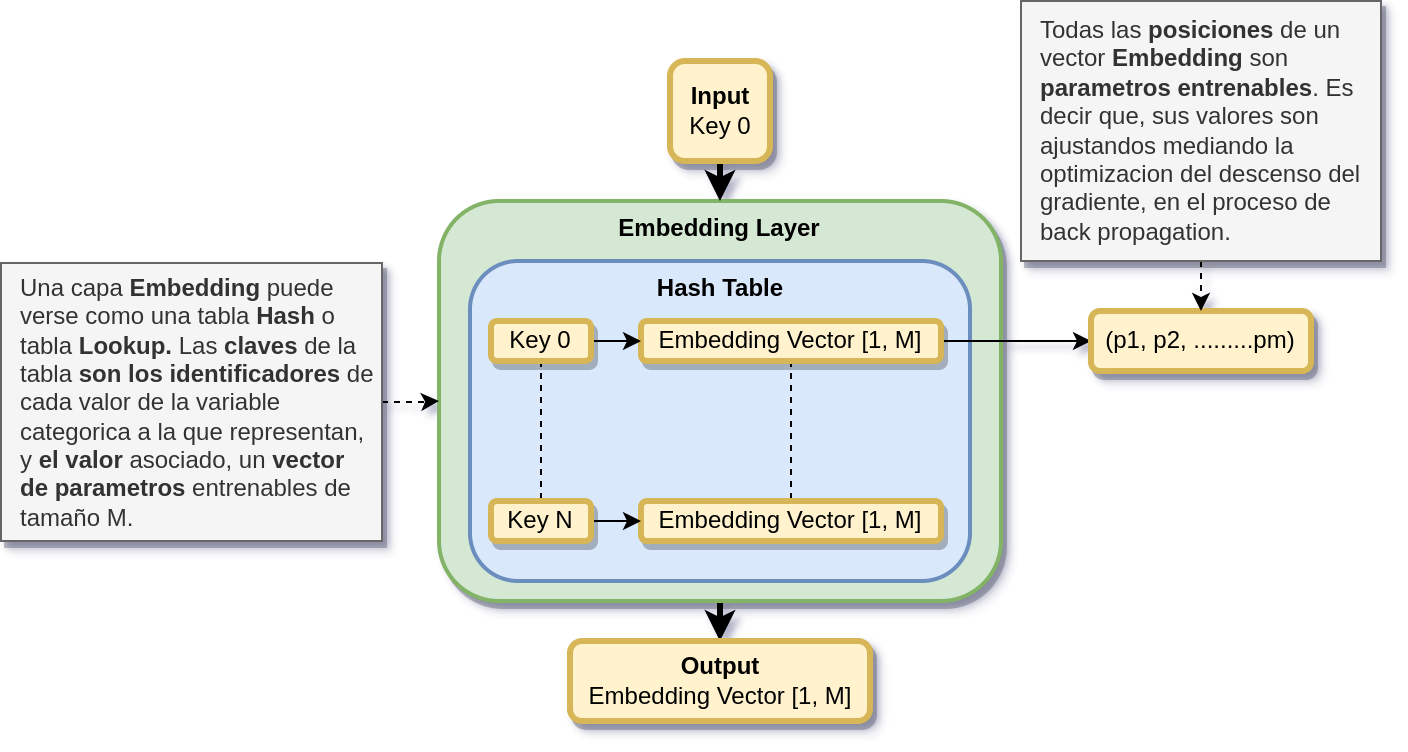
\includegraphics[width=13cm]{./images/Embedding-Layer.png}
	\caption{Esquema de una capa o módulo \textit{Embedding}.}
	\label{fig:embeddingLayer}
\end{figure}

\clearpage

\subsection{Arquitecturas Utilizadas}

En la sección anterior se explicó uno de los componentes básicos y más
utilizados en los modelos de recomendación basados en \textit{Deep Learning}. A
partir de este punto, se procederá a describir las arquitecturas utilizadas en
este trabajo.

\subsection{Factorización Matricial General (\textit{General Matrix Factorization o GMF})}

Esta es una arquitectura clásica en sistemas de recomendación basados en
filtros colaborativos. El algoritmo de factorización de matrices~\cite{afm}
funciona desacoplando la matriz de interacciones usuario-ítem en un producto
escalar de dos matrices regulares de baja dimensionalidad. Este algoritmo o
familia de algoritmos fue popularizado por primera por \textit{Simon Funk} en
la competencia \textit{Netflix prize}~\cite{netflixprize} en $2006$. La idea
principal del algoritmo es representar a usuarios e ítems en un espacio latente
de baja dimensionalidad. A partir del trabajo inicial realizado por
\textit{Funk} en $2006$, se han propuesto múltiples enfoques de factorización
de matrices para sistemas de recomendación, siento este el modelo mas simple y
efectivo.

Este modelo se puede construir fácilmente realizando el producto escalar de dos
matrices de vectores \textit{Embedding}, las cuales tiene una baja
dimensionalidad debido al principio de funcionamiento de los vectores
\textit{Embedding}. A continuación se puede ver un esquema del modelo, el cual
toma como entradas los identificadores de un usuario e ítem, luego resuelven
los vectores \textit{Embedding} correspondientes a ambos identificadores, y
finalmente se realiza el producto escalar de ambos vectores. Este producto
escalar tiene como resultado la calificación del usuario para el ítem dado. Por
otro lado, el algoritmo del optimización de gradiente descendente sera quien se
ocupe de ajustar los pesos de ambas matrices para que, dados los
identificadores de un usuario e ítem, se obtenga la calificación
correspondiente a la observación utilizada como ejemplo de entrenamiento.

\begin{figure}[h!]
	\centering
	\includegraphics[width=6cm]{./images/GMF.png}
	\caption{
		Esquema de un modelo \textit{General Matrix Factorization (GMF)}.
	}
	\label{fig:GMFModel}
\end{figure}

\clearpage

En términos matemáticos, este modelo realiza la siguiente operación en cada
paso hacia adelante (\textit{forward-pass}):

\begin{equation}
	\tilde{r}_{u, i} = V_u . V_i^{T}
\end{equation}
\begin{description}
	\item[Donde:]
\end{description}
\begin{itemize}
	\item $V_u$ es el vector \textit{embedding} correspondiente al usuario $u$.
	\item $V_i^{T}$ el vector \textit{embedding} correspondiente al ítem $i$.
	\item $ \tilde{r}_{u, i}$ es la predicción de la calificación realizada por el usuario $u$ al ítem $i$ (valor escalar).
\end{itemize}

En términos matriciales podemos verlo de la siguiente manera:

\begin{equation}
	\tilde{R} = U.I
\end{equation}
\begin{description}
	\item[Donde:]
\end{description}
\begin{itemize}
	\item $U\in\mathbb{R}^{u \times f}$ es la matriz de vectores \textit{Embedding} de usuarios,
	      la cuál tiene tantas filas $u$ como usuarios. $f$ es la dimensión del número de columnas
	      (también llamada factor latente) corresponde al tamaño seleccionado para los vectores \textit{Embedding}
	      (como ya se aclaro anteriormente, este es un hiper-parámetro a ajustar).
	\item $I\in\mathbb{R}^{f\times items}$ es la matriz de vectores \textit{Embedding} de ítems,
	      la cual tiene tantas filas como factores latentes (posiciones) en los vectores \textit{Embedding}, y
	      tantas columnas como ítems se tenga.
	\item $\tilde{R}\in\mathbb{R}^{usuarios \times items}$ es la matriz de calificaciones,
	      donde cada fila corresponde a un usuario y cada columna a un ítem.
\end{itemize}

El tamaño de la dimensión de factores latentes, como ya se vio anteriormente en
el apartado \textit{One-Hot vs. Embeddings}, es un hiper-parámetro mas a
ajustar. Se ha demostrado~\cite{embeddingsizedem} que realizar factorización de
matrices con un factor latente de tamaño 1 es equivalente a un modelo de
recomendación por popularidad, es decir que se recomiendan los ítems mas
populares sin tener en cuenta la personalización de las recomendaciones. Luego,
a medida que vamos incrementando el tamaño del factor latente, estas
recomendaciones serán cada vez más personalizadas, aumentando la calidad de las
mismas. Cuando el tamaño del factor latente es muy grande, el modelos a sobre
ajustar (\textit{overfitting}) y por ende la calidad de las recomendaciones
comenzara a empeorar. Para solucionar este problema, se suelen agregar términos
de regularización en la función de error a minimizar:

\begin{equation}
	\underset{H, W}{\operatorname{arg\,min } }\, \|R - \tilde{R}\|_{\rm F} + \alpha\|H\| + \beta\|W\|
\end{equation}
\begin{description}
	\item[Donde:]
\end{description}
\begin{itemize}
	\item $\|.\|_{\rm F}$ se define como [[norma matricial]]
	\item $\|H\|$ y $\|W\|$ pueden ser normas matriciales u otro tipo de norma dependiendo del sistema de recomendación.
\end{itemize}

\subsection{Factorización Matricial General con Sesgo
	(\textit{Biased General Matrix Factorization o B-GFM})}

El modelo \textit{GMF} de \textit{Simon Funk}~\cite{afm, dlwkrs}, visto en el
apartado anterior, realiza recomendaciones de muy buena calidad, pero tiene una
limitación: sólo utiliza interacciones usuario-ítem que tengan que ver con
valores numéricos referidos a interacciones explícitas, como calificaciones.
Los sistemas de recomendación modernos deben explotar todas las interacciones
posibles, tanto explícitas (calificaciones numéricas) como implícitas (compras,
vistas, favoritos, etc..). Para solucionar este nuevo problema, donde es
necesario usar cualquier tipo de interacción usuario-ítem (explicita o
implícita), se agrega un \textit{bias} o sesgo para los usuarios, y otro para
los ítems.

A Continuación se puede aprecia el diagrama del modelo, muy similar al diagrama
~\ref{fig:GMFModel}:

\begin{figure}[h!]
	\centering
	\includegraphics[width=11cm]{./images/Biased-GMF.png}
	\caption{
		Esquema de un modelo \textit{Biased General Matrix Factorization (B-GMF)}.
		A diferencia del modelo \textit{GMF}, este suma a la salida un \textit{bias}
		o sesgo por cada variable de entrada.
	}
	\label{fig:BiasedGMFModel}
\end{figure}

En este caso se agregan dos nuevas capas \textit{Embedding}, las cuales
representa a los sesgos de usuarios e ítems respectivamente. El tamaño de los
factores latentes o vectores \textit{Embedding} correspondiente a cada
\textit{bias} o sesgo es $1$, dado que son valores escalares. Finalmente, luego
de calcular el producto escalar, se suman los factores latentes resultado de
ambas capas \textit{Embedding} correspondiente a los \textit{bias} o sesgos.

\clearpage

\subsection{Factorización Matricial mediante Redes Neuronales
	(\textit{Neural Network Matrix Factorization o NN-FM})}

En los enfoques anteriormente vistos (\textit{GFM} y \textit{Biased GFM}),
dadas dos matrices de baja dimensionalidad se realiza un producto escalar y se
suman sesgos, dependiendo del caso, para calcular o inferir la calificación de
un usuario para un ítem dado. Estos modelos, como ya se explico anteriormente,
aprenden los pesos o parámetros de los vectores \textit{Embedding} en el
proceso se entrenamiento.

El enfoque de {\textit{NN-MF}}~\cite{nnfm}~\cite{ncf} es levemente distinto. En
este caso se reemplaza el producto interno, el cual podemos pensarlo como
conocimiento a priori del problema, por otra función desconocida, que sera la
que aprenderá el modelo a partir de las observaciones suministradas en el
entrenamiento. En particular, se remplaza el producto escalar sumado a los
sesgos, por una red neuronal multi-capa de capas densas o \textit{fully
	connected}. De esta forma, el modelo no solo aprender los parámetros de los
vectores \textit{embedding}, sino también los pesos de la red multi-capa. En
definitiva el modelo aprende cual es la mejor función para predecir las
calificaciones del usuario.

El uso de redes neuronales presenta una ventaja significativa: la posibilidad
de utilizar múltiples variables como entrada, no limitándose únicamente a las
variables categóricas usuario e ítem. Es precisamente en esta característica
donde radica su mayor potencial. No obstante, es importante mencionar que este
modelo muestra una ligera disminución en la precisión de sus predicciones en
comparación con modelos anteriores.

A continuación podemos ver un esquema del modelo, muy similar a \textit{GFM}
como ya se dijo, con la diferencia que tenemos una red multi capa en vez de un
producto escalar.

\begin{figure}[h!]
	\centering
	\includegraphics[width=6cm]{./images/NN-MF.png}

	\caption{
		Esquema de un modelo \textit{Neural Network Matrix Factorization (NN-MF)}.
	}
	\label{fig:NNMFModel}
\end{figure}

Para comenzar, el modelo tiene como entradas independientes los identificadores
de usuarios e ítems. Cada capa \textit{Embedding} retorna el correspondiente
vector \textit{embedding} asociado a estos identificadores. A continuación, el
bloque \textit{Flatten} toma ambos vectores y produce uno nuevo mediante su
concatenación. Este vector resultante se convierte en la entrada de una red
multi-capa.

Es importante destacar que la red multi-capa tendrá tantas entradas como
dimensiones posea este nuevo vector combinado. La cantidad de capas y el número
de neuronas por capa son hiper-parámetros que se ajustarán durante el proceso
de optimización. Por esta razón, no se especifica un número fijo de capas o
neuronas por capa.

Cada capa, excepto la última, utiliza la función de activación \textit{ReLU},
mientras que la capa final emplea una activación \textit{Lineal}, similar a una
regresión lineal. Esto se debe a que el objetivo es predecir las
calificaciones, las cuales tienen un rango de valores reales entre $0.5$ y $5$.
Es importante señalar que se está considerando utilizar una activación
\textit{Softmax} en lugar de una activación \textit{Lineal} en la última capa,
lo que permitiría abordar el problema como uno de clasificación.

\clearpage

\subsection{Máquinas de Factorización (\textit{FM})}

Antes de introducir el modelo de máquinas de factorización profundas
(\textit{DeepFM}) se comenzara explicando uno de sus componentes mas
importantes: las máquinas de factorización~\cite{didlfm, zhangdive}.

Las máquina de factorización propuestas por \textit{Steffen Rendle} en 2010
~\cite{fm}, son algoritmos supervisados que puede ser utilizados para tareas de
clasificación, regresión y tareas de ranking como sucede en el ámbito de los
sistemas de recomendación. Rápidamente se convirtieron en un método popular
para hacer predicciones y recomendaciones. La máquina de factorización es una
generalización de un modelo lineal y un model de factorización de matrices, mas
aun, recuerdan mucho a un máquina de soporte vectorial \textit{(SVM)} que
utiliza un kernel polinomial.

A continuación, se define el modelo formalmente:

\begin{itemize}
	\item $x\in\mathbb{R}^{d}$ es un vector de \textit{features} donde cada una de sus
	      componentes representa a una variable del \textit{dataset}, siendo $d$
	      la cantidad de variables. En nuestro caso,
	      $x\in\mathbb{R}^{2}$ ya que tenemos dos variables, usuarios e ítems.
	\item $y\in\mathbb{R}$ es la variable \textit{target} o resultado a predecir.
	      Dado el dominio del \textit{dataset} seleccionado, seria la
	      calificación del usuario.
\end{itemize}

Luego, podemos definir el modelo para una máquina de factorización de grado $2$
de la siguiente forma:

\begin{equation}
	\hat{y}(x) = \mathbf{w}_0 + \sum_{i=1}^d \mathbf{w}_i x_i + \sum_{i=1}^d\sum_{j=i+1}^d
	\langle\mathbf{v}_i, \mathbf{v}_j\rangle x_i x_j
\end{equation}
\begin{description}
	\item[Donde:]
\end{description}
\begin{itemize}
	\item $d$ es la cantidad de \textit{features} o variables a utilizar.
	      Para el caso de estudio en este trabajo $d=2$ (usuarios e ítems).
	\item $\mathbf{w}_0 \in \mathbb{R}$ es el \text{bias} o intercepto del modelo.
	\item $\sum_{i=1}^d \mathbf{w}_i x_i$: Esta es la parte lineal del modelo. Aquí,
	      $x_i$ representa el valor del \textit{feature} $i$-ésimo. $\mathbf{w}_i$ es
	      el peso asociado al \textit{feature} $i$-ésimo, que determina la influencia
	      de ese \textit{feature} en la predicción. Multiplicamos el valor de cada
	      \textit{feature} $x_i$ por su peso correspondiente $\mathbf{w}_i$ y sumamos
	      todas estas contribuciones para obtener la parte lineal de la predicción.
	\item $\sum_{i=1}^d\sum_{j=i+1}^d \langle\mathbf{v}_i, \mathbf{v}_j\rangle x_i x_j$:
	      Esta es la parte de factorización del modelo. Donde, $\langle\mathbf{v}_i,
		      \mathbf{v}_j\rangle$ es el producto interno (o producto escalar) entre
	      los vectores $\mathbf{v}_i$ y $\mathbf{v}_j$. Cada vector $\mathbf{v}_i$
	      representa una factor latente o \textit{Embedding} del \textit{feature}
	      $i$-ésimo. Estos vectores capturan interacciones no lineales entre
	      características y se utilizan para modelar relaciones más complejas
	      entre ellas. Similar a la parte lineal, multiplicamos los valores
	      de las características $x_i$ y $x_j$ por el producto interno
	      $\langle\mathbf{v}_i, \mathbf{v}_j\rangle$ y sumamos todas las contribuciones
	      para obtener la parte de factorización de la predicción.

\end{itemize}

En resumen, la expresión completa $\hat{y}(x)$ representa la estimación de la
variable dependiente $\hat{y}$ basada en la entrada $x$, utilizando una
combinación lineal de los pesos de las características y una suma de productos
internos entre los vectores de características latentes para capturar
interacciones no lineales entre las características. Este modelo es comúnmente
utilizado en el campo del aprendizaje automático para problemas de regresión y
clasificación.

De esta forma los dos primeros términos corresponden al modelo de regresión
lineal y el último término es una extensión del modelo de factorización
matricial. Si la variable $i$ representa un ítem y la variable $j$ a un
usuario, el tercer término es el producto escalar entre los vectores
\textit{embedding} de usuario $u$ y ítem $i$. Por otro lado, vale la pena
aclarar que este método también puede generalizar en órdenes superiores al
grado 2, sin embargo, la estabilidad numérica podría disminuí la generalización
del método.

Al aplicar un método de optimización con las máquinas de factorización, como
puede ser el método del gradiente descendente, se puede llegar fácilmente a una
complejidad del orden $\mathcal{O}(kd^2)$, ya que se deben calcular todas las
interacciones de a pares. Para resolver este problema de \textit{performance},
podemos reorganizar el tercer término del método, Esto reduce en gran medida el
costo de cálculo, llevándolo a una complejidad de tiempo de orden lineal
$\mathcal{O}(kd)$. A continuación se describen los pasos para bajar el nivel de
complejidad del método:

\begin{equation}
	\begin{split}
		&=\sum_{i=1}^d \sum_{j=i+1}^d \langle\mathbf{v}_i, \mathbf{v}_j\rangle x_i x_j \\
		&= \frac{1}{2} \sum_{i=1}^d \sum_{j=1}^d\langle\mathbf{v}_i, \mathbf{v}_j\rangle x_i x_j - \frac{1}{2}\sum_{i=1}^d \langle\mathbf{v}_i, \mathbf{v}_i\rangle x_i x_i \\
		&= \frac{1}{2} \big (\sum_{i=1}^d \sum_{j=1}^d \sum_{l=1}^k\mathbf{v}_{i, l} \mathbf{v}_{j, l} x_i x_j - \sum_{i=1}^d \sum_{l=1}^k \mathbf{v}_{i, l} \mathbf{v}_{i, l} x_i x_i \big)\\
		&=  \frac{1}{2} \sum_{l=1}^k \big ((\sum_{i=1}^d \mathbf{v}_{i, l} x_i) (\sum_{j=1}^d \mathbf{v}_{j, l}x_j) - \sum_{i=1}^d \mathbf{v}_{i, l}^2 x_i^2 \big ) \\
		&= \frac{1}{2} \sum_{l=1}^k \big ((\sum_{i=1}^d \mathbf{v}_{i, l} x_i)^2 - \sum_{i=1}^d \mathbf{v}_{i, l}^2 x_i^2)
	\end{split}
\end{equation}

Con esta reformulación del último termino, la complejidad del método se reduce
considerablemente. Además, para las variables ralas, solo se deben computar los
valores distintos de cero, para que la complejidad general sea lineal.
Finalmente, la expresión del método aplicando esta reformulación queda como
sigue:

\begin{equation}
	\hat{y}(x) = \mathbf{w}_0 + \sum_{i=1}^d \mathbf{w}_i x_i + \frac{1}{2} \sum_{l=1}^k \big ((\sum_{i=1}^d \mathbf{v}_{i, l} x_i)^2 - \sum_{i=1}^d \mathbf{v}_{i, l}^2 x_i^2)
\end{equation}

\clearpage

\subsection{Máquinas de factorización profundas (\textit{DeepFM})}

Hasta aquí, a grandes rasgos, todos los modelos expuestos tratan de captar el
comportamiento de las interacciones o correlación usuario-ítems, ya sean
implícitas o explicitas. A pesar de este gran progreso, los métodos expuestos
anteriormente (exceptuando las máquinas de factorización) parecen tener un
fuerte sesgo al predecir las interacciones o correlaciones de bajo y alto
orden, requiriendo en algunos casos realizar ingeniería de \textit{features}
para disminuir estos sesgos.

El modelo de máquinas de factorización profundas
(\textit{DeepFM})~\cite{dfmpaper, didldfm} o maquina de factorización basada en
\textit{Deep Learning}, mejora el aprendizaje de las interacciones o
correlaciones de bajo y alto orden. Este modelo combina máquinas de
factorización y \textit{Deep Learning} en una nueva arquitectura de red
neuronal, la cual captura estas correlaciones. Por otro lado, es una evolución
del modelo \textit{Wide and Deep}~\cite{wideanddeeppaper} de \textit{Google},
el cual es un ensamble de dos modelos: uno lineal, que captura las
interacciones o correlaciones de alto orden y una red neuronal perceptron
multi-capa o \textit{Multi-Layer Perceptron (MLP)}, la cual captura correlación
de mas bajo orden (aquellas mas complejas).

A continuación de puede visualizar un diagrama de bloques de alto nivel del
modelo:

\begin{figure}[h!]
	\centering
	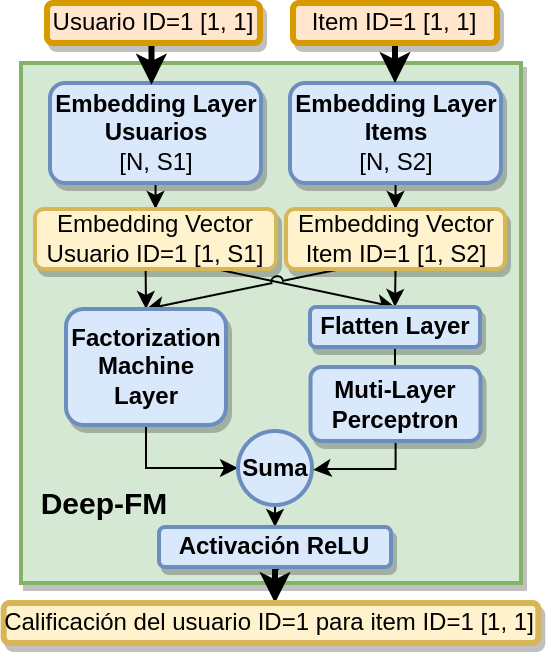
\includegraphics[width=6cm]{./images/Deep-MF.png}
	\caption{
		Esquema de un modelo \textit{Deep Factorization Machine (DeepFM)} o maquina
		de factorización basada en \textit{Deep Learning}.
	}
	\label{fig:DeepMFModel}
\end{figure}

Donde se puede apreciar que las entradas del modelo son las variables
categóricas correspondiente a usuarios e ítems, como en los modelos previamente
visto. Dado un identificador de usuario e ítem, se resuelve sus correspondientes
vectores \textit{Embedding}, los cuales se convierten en entradas para los
siguientes dos bloques. Uno de los bloques intermedios, no es mas que una red
neuronal multi capa con capas densas o \textit{fully connected}. Por el otro
lado, ambos vectores se toman como entrada a la máquina de factorización. Las
salidas de ambos bloques intermedios, de valores escalares, se suman y se pasan
por una activación \textit{ReLU}. Para el caso de estudio de este trabajo, las
salidas o calificaciones toman valores mayores a cero, por esta cuestión es mas
adecuado usar una activación \textit{ReLU} frente a una lineal.

\section{Métricas}
\label{sec:metrics}

Para medir y comparar el grado de exactitud de los modelos seleccionados, tanto
en el conjunto de validación como entrenamiento, se han seleccionado dos
métricas:

\begin{itemize}
	\item \textit{Root Mean Square Error (RMSE)}: Es la raíz cuadrada del error
	      cuadrático medio.
	\item \textit{Mean Average Precision at k (mAP@k)}: Es la media del
	      promedio de la precisión  para un tamaño K de observaciones.
\end{itemize}

\subsection{\textit{Root Mean Square Error (RMSE)}}
\label{sec:rmse_ref}

Dado que todos los modelos que se evaluaron en este trabajo tiene como salida
una variable real (Calificación de los usuarios para un ítem), es posible
utilizar \textit{RMSE}. Esta métrica es utilizada en problemas de regresión
donde la salida del modelo es una variable numérica real.

Si bien esta métrica no es la métrica por excelencia a usar en el ámbito de
sistemas de recomendación, ayuda a comprender cuales el grado de ajuste de los
modelos y puede servir como una métrica complementaria al momento de evaluar
los mismos.

\begin{description}
	\item[Definición:]
\end{description}

\begin{equation}
	\operatorname{RMSE}=\sqrt{\frac{1}{N} \sum_{i=1}^N (y_i - \hat y_i)^2}
\end{equation}

\begin{description}
	\item[Donde:]
\end{description}

\begin{itemize}
	\item $y_i$ es el true value o verdad de campo de la observación.
	\item $\hat y_i$ es la predicción realizada por el modelo predictor.
	\item $N$ es el numero de observaciones sobre las que se realizo la predicción del modelo.
\end{itemize}

\subsection{\textit{Mean Average Precision at k (mAP@k)}}
\label{sec:map_ref}

\textit{Mean Average Precision at k (mAP@k)} o media del promedió de la
precisión para K observaciones, es una de las métricas mas usada
para evaluar sistemas de recomendación~\cite{map_at_k_1, map_at_k_2, map_at_k_3}.

Antes de comenzar, definamos a los sistemas de recomendación en términos de sus
entradas y salida, donde:

\begin{itemize}
	\item Entradas: Como entradas tenemos el identificador del usuario al cual queremos
	      presentarle recomendaciones y otro parámetro opcional que podría ser el
	      identificador de un ítem. ¿Por que opcional? Bueno, en general si no se
	      especifica un identificador de ítem, igualmente es posible encontrar cuales son
	      los ítems de mayor preferencia para el usuario y luego recomendar nuevos ítems
	      en base a este ítem inicial. Por otro lado, si ya se cuenta con un
	      identificador de ítem, se puede recomendar ítems similares a este. Este último
	      caso es muy común cuando un usuario navega al detalle de un producto en un
	      \textit{e-commerce}. En esta instancia, ya se conoce el identificador del
	      usuario e ítem. Finalmente, se recomiendan ítems similares al ítem visualizado.
	\item Salidas: Es una lista de ítems recomendados similares a otro ítem (entrada del
	      modelo) ordenados descendente-mente por la calificación predicha por el modelo
	      para el usuario en cuestión (entrada del modelo).
\end{itemize}

Entonces, se podría decir que dada la salida de un sistema de recomendación, si
encontramos en las primeras posiciones de la lista aquellos ítems con mayor
calificación predicha, seria un buen indicador de que el modelo es preciso al
momento de recomendar. En palabras mas simples, se desea que los primeros ítems
de la lista de recomendaciones sean de mayor agrado para el usuario.

¿Finalmente, como funciona esta métricas? La métrica
\textit{mAP\makeatletter@k} funciona de la siguiente forma: Supongamos que tenemos
un usuario y una lista K de ítems a recomendar. En base
a estas entradas el modelo de recomendación predice las calificaciones de cada
ítem para el usuario dado. Luego, podemos ordenar la lista de ítems
descendente-mente de acuerdo a las calificaciones predichas por el modelo.

Teniendo esta lista, se puede calcular el promedio de la predicción
\textit{mAP\makeatletter@k} sobre los K ítems de la lista.

Esta métrica es utilizada en problemas de clasificación pero también se puede
utilizar en problemas donde el modelo produce una salida numérica como en este
caso. Los niveles o clases a utilizar dependen mucho de que se quiera evaluar.
Supongamos, en este caso particular, que queremos medir con que precisión
aparecen las puntuaciones entre 4 y 5 en las primera posiciones de la lista.
Para este fin se utilizara la métricas \textit{mAP\makeatletter@k}.

\begin{description}
	\item[Promedio de la precisión sobre una lista de K elementos
	\textit{AP\makeatletter@k}:]
\end{description}
\begin{equation}
	\begin{split}
		& \operatorname{AP\makeatletter@k}=\frac{1}{N(k)} \sum_{i=1}c \frac{ TP(i)}{i}, \\
		& \\
		& \operatorname{N(k)} = min(k, TP_{total}) \\
	\end{split}
\end{equation}
\begin{description}
	\item[Donde:]
\end{description}
\begin{itemize}
	\item $i$ es la posición del ítem $i^\mathrm{th}$ en la lista de $k$ elementos. $i$  toma valores entre $1$ y $k$.
	\item $TP_i$ es 1 si la precisión y el valor verdadero concuerdan.
	\item $N(k)$ es el mínimo entre el tamaño de la lista y la cantidad de $TP_{total}$ encontrados en esa lista.
\end{itemize}

Por ejemplo, si se quiere saber con que precisión aparecen ítems con
calificaciones entre 4 y 5 puntos en las primeras posiciones de la lista:

\begin{itemize}
	\item Si $TP_i$ es igual a $1$, entonces la calificación en la posición
	      $i^\mathrm{th}$ se encuentra entre los 4 y 5 punto.
	\item Si $TP_i$ es igual a $0$, entonces la calificación en la posición
	      $i^\mathrm{th}$ NO se encuentra entre los 4 y 5 punto.
\end{itemize}

De esta forma, se esta transformando la salida del modelo en una lista de
valores binarios. Donde la clase 1 indica que se cumple con la condición
esperada y la clase 0 lo contrario.

Luego se realiza el calculo de \textit{AP\makeatletter@k} para cada usuario del
\textit{dataset} de validación y finalmente se calcula la media:

\begin{description}
	\item[Media del promedio de la precisión sobre una lista de K elementos
	\textit{mAP\makeatletter@k}:]
\end{description}
\begin{equation}
	\operatorname{mAP\makeatletter@k}=\frac{1}{N} \sum_{i=1}^N AP\makeatletter@k_i
\end{equation}

De esta forma, la métrica \textit{mAP\makeatletter@k} da una noción del grado
de precisión en que aparecen ítems con mayor puntuación en las primeras
posiciones de una lista de tamaño $k$. Cabe aclarar, que la condición
\textit{ítems con mayor puntuación} es arbitraria, aun que al ser una
condición, podríamos intercambiarla por cualquier otro criterio. Por ejemplo,
ítems con las peores puntuaciones (entre 1 y 2 puntos), ítems con puntuaciones
medias, ítems con mas de 3 puntos, menos de 3 puntos, etc...

\chapter{Experimentos}

Con el propósito de comparar todos los modelos implementados, se empleó el
mismo conjunto de datos (\textit{dataset}). Se tomó una muestra con un tamaño
adecuado para garantizar resultados sólidos, al mismo tiempo que se evitó el
sobreajuste (\textit{overfitting}) en aquellos modelos propensos a esta
problematica. Adicionalmente, se realizó una modificación en el modelo
\textit{KNN} para almacenar sus resultados en una memoria \textit{cache}.
Mediante este enfoque, al momento de seleccionar muestras del conjunto de
validación, se realiza una única inferencia del rating para cada par
usuario-ítem, lo que conlleva una reducción significativa en el tiempo total de
predicción del modelo.

Por otra lado, es importante señalar que debido a la propensión de los modelos
hacia la variabilidad o varianza en sus predicciones, se llevó a cabo un
muestreo de $5.000$ inferencias para cada modelo en el conjunto de validación,
considerando cada métrica utilizada. Posteriormente, se generó un histograma
que representa la distribución de estas métricas, así como un diagrama de caja
(\textit{boxplot}) para obtener una comprensión precisa del valor promedio y la
dispersión.

A continuación se describen los resultados de todos los modelos comparados
mediando las métricas \textit{mAP\makeatletter@k} y \textit{RMSE}.

\section{
  Algoritmo de los K vecinos cercanos
  (\textit{K-Nearest-Neighbor} o \textit{KNN}) }

A continuación se describen los resultados de las métricas de evaluación sobre
la familia de modelos \textit{KNN}: \textit{KNN User Based}, \textit{KNN Item
	Based} y el ensamble de ambos modelos.

\subsection{
	Algoritmo de los K vecinos cercanos basado
	en usuarios (\textit{KNN User Based})
}

\begin{figure}[!htb]
	\centering
	\includegraphics[width=15cm]{./images/metrics-knn-user-based-mapk.png}
	\caption{
		Esta gráfica describe la distribución de valores de la métrica
		\textit{mAP@5(4,5)} evaluada en el conjunto de observaciones de
		validación. Se realizo un muestreo de N inferencias del modelo
		\textit{KNN User Based} sobre las observaciones de validación.
	}
	\label{fig:knnUserMAP}
\end{figure}

En la figura~\ref{fig:knnUserMAP} se describe la distribución de valores de la
métrica \textit{mAP@5(4,5)} evaluada en el conjunto de observaciones de
validación. Se pueden apreciar por lo menos $3$ valores atípicos en el extremo
derecho. Esto advierte cierto grado de sobre ajusto del modelo, que ajusta muy
bien sobre estas observaciones atípicas.

El valor medio de la predicción es de $0.381943$. El $50$\% de las
observaciones se encuentran entre $0.367234$ y $0.396652$ respectivamente, con
una dispersión de $0.014709$. La media es muy cercana a la mediana, con una
diferencia de $0.000646$; indicando una baja influencia de los valores atípicos
sobre la media. En parte, esto ultimo se debe al gran tamaño de la muestra
tomada.

La distribución presenta una forma mesocúrtica, dado que presenta una curtosis
moderada, lo que significa que sus colas o extremos son relativamente menos
pesadas que en una distribución leptocúrtica (con exceso de curtosis) y más
pesadas que en una distribución platicúrtica (con poca curtosis).

\begin{figure}[!htb]
	\centering
	\includegraphics[width=15cm]{./images/metrics-knn-user-based-RMSE.png}
	\caption{
		Esta gráfica describe la distribución de valores de la métrica
		\textit{RMSE} evaluada en el conjunto de observaciones de
		validación. Se realizo un muestreo de N inferencias del modelo
		\textit{KNN User Based} sobre las observaciones de validación.
	}
	\label{fig:knnUserRMSE}
\end{figure}

En la figura~\ref{fig:knnUserRMSE} se describe la distribución de valores de la
métrica \textit{RMSE} evaluada en el conjunto de observaciones de validación.

Se aprecia por lo menos $1$ valor atípicos en el extremo derecho. Sin embargo
esto no parece afectar a la forma de la distribución. La distribución esta
sesgada a izquierda. Este sesgo arrastra a la media y mediana hacia valores mas
bajos del error, siendo un comportamiento deseable. Es decir, cuando mas
probabilidad se acumule a izquierda mayor sera la frecuencia de ocurrencia para
valores bajos del error.

El valor medio del error es de $2.9523$. El $50$\% de las observaciones se
encuentran entre $2.9361$ y $2.9684$ respectivamente, con una dispersión de
$0.016170$. La media es muy cercana a la mediana, con una diferencia de
$0.000356$; también indicando una baja influencia de los valores atípicos sobre
la media.

\clearpage

\subsection{
	Algoritmo de los K vecinos cercanos basado
	en ítems (\textit{KNN Item Based})
}

\begin{figure}[!htb]
	\centering
	\includegraphics[width=15cm]{./images/metrics-knn-item-based-mapk.png}
	\caption{
		Esta gráfica describe la distribución de valores de la métrica
		\textit{mAP@5(4,5)} evaluada en el conjunto de observaciones de
		validación. Se realizo un muestreo de N inferencias del modelo
		\textit{KNN Item Based} sobre las observaciones de validación.
	}
	\label{fig:knnItemMAP}
\end{figure}

En la figura~\ref{fig:knnItemMAP} se describe la distribución de valores de la
métrica \textit{mAP@5(4,5)} evaluada en el conjunto de observaciones de
validación. Se pueden apreciar valores atípicos a ambos extremos. Fuera de
esto, la distribución tiene una forma gaussiana casi perfecta, indicando la
ausencia de sesgos a derecha o izquierda.

El valor medio de la precisión es de $0.380327$. El $50$\% de las observaciones
se encuentran entre $0.365618$ y $0.395036$ respectivamente, con una dispersión
de $0.014056$. La media es muy cercana a la mediana con una diferencia de
$0,000043$, indicando una baja influencia de valores atípicos sobre la misma.
La distribución presenta una forma mesocúrtica.

\clearpage

\begin{figure}[!htb]
	\centering
	\includegraphics[width=15cm]{./images/metrics-knn-item-based-RMSE.png}
	\caption{
		Esta gráfica describe la distribución de valores de la métrica
		\textit{RMSE} evaluada en el conjunto de observaciones de
		validación. Se realizo un muestreo de N inferencias del modelo
		\textit{KNN Item Based} sobre las observaciones de validación.
	}
	\label{fig:knnItemRMSE}
\end{figure}

En la figura~\ref{fig:knnItemRMSE} se describe la distribución de valores de la
métrica \textit{RMSE} evaluada en el conjunto de observaciones de validación.
Se aprecia por lo menos $3$ valor atípicos en el extremo derecho. La
distribución esta levemente sesgada a izquierda.

El valor medio del error es de $3.103917$. El $50$\% de las observaciones se
encuentran entre $3,088942$ y $3,118892$ respectivamente, con una dispersión de
$0,014975$. La media es muy cercana a la mediana con una diferencia de
$0,000151$, indicando una baja influencia de valores atipicos sobre la misma.

Se aprecia un mayor error en las predicciones del modelo \textit{KNN Item
	Based} ($3.103917$) en comparación con el modelo \textit{KNN User Based}
($2.952305$).

\subsection{Modelo ensamble de los algoritmos de los K
	vecinos cercanos basados en usuarios e ítems
	(\textit{KNN User-Item Based Ensemble})
}

\begin{figure}[!htb]
	\centering
	\includegraphics[width=15cm]{./images/metrics-knn-ensemple-mapk.png}
	\caption{
		Esta gráfica describe la distribución de valores de la métrica
		\textit{mAP@5(4,5)} evaluada en el conjunto de observaciones de
		validación. Se realizo un muestreo de N inferencias del modelo
		\textit{KNN User-Item Based Ensemble} sobre las observaciones
		de validación.
	}
	\label{fig:knnEnsempleMAP}
\end{figure}

En la figura~\ref{fig:knnEnsempleMAP} se observa la distribución de valores de
la métrica \textit{mAP@5(4,5)} evaluada en el conjunto de observaciones de
validación. Se pueden apreciar valores atípicos a ambos extremos y un leve
sesgo a izquierda, debido al aporte del modelos basado en ítems.

Por otro lado, la distribución tiene colas mas pesadas en esta versión de
ensamble de ambos modelos (basado en usuarios e ítems).

El valor medio de la precisión es de $0.384819$, ligeramente mayor a la
precisión de ambos modelos (basado en usuarios e ítems). El desvío también
aumenta de $0.014$ a $0.015$.

\begin{figure}[!htb]
	\centering
	\includegraphics[width=15cm]{./images/metrics-knn-ensemple-RMSE.png}
	\caption{
		Esta gráfica describe la distribución de valores de la métrica
		\textit{RMSE} evaluada en el conjunto de observaciones de
		validación. Se realizo un muestreo de N inferencias del modelo
		\textit{KNN User-Item Based Ensemble} sobre las observaciones
		de validación.
	}
	\label{fig:knnEnsempleRMSE}
\end{figure}

En la figura~\ref{fig:knnEnsempleRMSE} se aprecia la distribución de valores de
la métrica \textit{RMSE} evaluada en el conjunto de observaciones de
validación.

Se observa por lo menos $1$ valor atípicos en el extremo derecho. La
distribución esta levemente sesgada a izquierda.

El valor medio del error es de $2.917146$ con una dispersión de $0.015642$, en
ambos casos menores a las mediciones sobre ambos modelos por separado.

En resumen, el ensamble de ambos modelos obtiene una mayor precisión y un menor
porcentaje de error al realizar predicciones.

\clearpage
\section{Factorización Matricial General (\textit{General Matrix Factorization o GMF})}

A continuación, se presentan las curvas de error (\textit{RMSE}) del modelo
\textit{GMF} al ser evaluado en los conjuntos de validación y entrenamiento:

\begin{figure}[ht]
	\centering
	\includegraphics[width=13cm]{./images/metrics-GFM-train-val-loss.png}
	\caption{
		Esta gráfica describe el nivel de error sobre los conjuntos
		de observaciones de entrenamiento y validación durante el
		entrenamiento del modelo \textit{GFM}. Cada \textit{epoch} o época
		indica una iteración de entrenamiento del modelo sobre el conjunto
		completo de entrenamiento.
	}
	\label{fig:gmfLoss}
\end{figure}

En la figura~\ref{fig:gmfLoss} se puede observar que desde la iteración
(\textit{epoch}) primera a la cuarta (aproximadamente), el modelo está
aprendiendo a generalizar a partir de los datos de entrenamiento. En esta etapa
inicial, el modelo no tuvo suficiente tiempo para ajustarse completamente a las
observaciones de entrenamiento. Por lo tanto, puede haber menos sobre ajuste y,
en algunos casos, el modelo podría generalizar mejor a los datos de validación
que a los datos de entrenamiento.

A medida que el modelo sigue entrenando, tiene la capacidad de capturar más
detalles y patrones específicos de las observaciones de entrenamiento. Esto
puede llevar a un ajuste excesivo a esos detalles, lo que hace que el error en
los datos de entrenamiento disminuya. Sin embargo, estos detalles pueden no ser
generalizables y pueden causar que el modelo se desempeñe peor con
observaciones nuevas (validación). En consecuencia, el error en el conjunto de
validación puede comenzar a aumentar a medida que el modelo se sobreajusta a
los datos de entrenamiento. Finalmente, se puede observar que el modelo
sobreajusta con una diferencia sostenida entre validación y entrenamiento. Mas
alla del sobreajuste, la curva de validación dejar de descender luego de las
$20$ iteraciones. En este caso se opta por frenar el entrenamiento en la
iteracion 4, donde el modelo todavía no llega al sobreajuste y donde puede
generalizar mejor.

\clearpage

A continuación, se describe la distribución de la métrica \textit{mAP@5(4,5)}
del modelo evaluado sobre el conjunto de validación:

\begin{figure}[h!]
	\centering
	\includegraphics[width=15cm]{./images/metrics-GFM-mapk.png}
	\caption{
		Esta gráfica describe la distribución de valores de la
		métrica \textit{mAP@5(4,5)} evaluado en el conjunto de observaciones
		de validación, luego de N procesos de entrenamiento del modelo
		\textit{GFM} sobre las observaciones de entrenamiento.
	}
	\label{fig:gmfMAP}
\end{figure}

En la figura~\ref{fig:gmfMAP} se pueden apreciar al menos $1$ valor atípicos en
el extremo derecho. Fuera de esto la distribución tiene una forma gaussiana
casi perfecta, indicando la ausencia de sesgos a derecha o izquierda. El valor
medio de la precisión es de $0.406646$ con una dispersión de $0.012513$. La
media esta muy cercana a la mediana con una diferencia de $0.000224$, esto
indica una baja influencia de de valores atípicos sonre la media. La
distribución presenta una forma mesocúrtica.

\begin{figure}[h!]
	\centering
	\includegraphics[width=15cm]{./images/metrics-GFM-RMSE.png}
	\caption{
		Esta gráfica describe la distribución de valores de la métrica
		\textit{RMSE} evaluado en el conjunto de observaciones de validación,
		luego de N procesos de entrenamiento del modelo \textit{GFM} sobre
		las observaciones de entrenamiento.
	}
	\label{fig:gmfRMSE}
\end{figure}

En la figura~\ref{fig:gmfRMSE} se describe la distribución de valores de la
métrica \textit{RMSE} evaluada en el conjunto de observaciones de validación.
Se aprecia por lo menos $1$ valor atípicos en el extremo izquierda. No se
aprecia sesgo a simple vista. El valor medio del error es de $ 0.982894$ con
una dispersión de $0.009419$.

En resumen, al comparar las métricas entre la familia de modelos \textit{KNN} y
el modelo \textit{GMF}, se observa un incremento en la precisión de
aproximadamente entre un $1.5\%$ y un $2\%$. Además, la dispersión de la
precisión también disminuye en $0.002$ puntos. Estos resultados sugieren que el
modelo \textit{GMF} es una opción más prometedora que \textit{KNN}, ya que
demuestra una mayor precisión y un menor error en las predicciones.

\clearpage

\section{Factorización Matricial General con Sesgo
  (\textit{Biased General Matrix Factorization o B-GFM})}

A continuación, se presentan las curvas de error (\textit{RMSE}) del modelo
\textit{B-GMF} al ser evaluado en los conjuntos de validación y entrenamiento:

\begin{figure}[h!]
	\centering
	\includegraphics[width=13cm]{./images/metrics-BGFM-train-val-loss.png}
	\caption{
		Esta gráfica describe el nivel de error sobre los conjuntos
		de observaciones de entrenamiento y validación durante el entrenamiento
		del modelo \textit{B-GFM}. Cada epoch o época indica una iteración de
		entrenamiento del modelo sobre el conjunto completo de entrenamiento.
	}
	\label{fig:bGMFLoss}
\end{figure}

En la figura~\ref{fig:bGMFLoss} se aprecia un comportamiento muy similar al
modelo \textit{GMF}. La principal diferencia radica en el punto de cruce entre
las curvas. El modelo \textit{B-GMF} parece generalizar con un error menor que
el modelo \textit{GMF}. Aqui en donde se aprecia que la leve modificación al
sumar un sesgos (uno para usuarios y otro para ítems) disminuje el error sobre
el punto de mayor generalización del modelo.

Este fenomeno ocurre al incorporar los sesgos, el modelo captura efectos que
influyen en las predicciones y que no son explicados completamente por la
descomposición de matrices.

La descomposición de matrices realizada por el modelo \textit{GMF}, intenta
capturar las interacciones entre usuarios e ítems basándose en las
calificaciones históricas de los usuarios para los ítems. Pero hay factores
adicionales que pueden influir en las preferencias de los usuarios y en cómo
califican los ítems. Estos factores pueden no estar directamente relacionados
con las interacciones pasadas, pero aún así afectan las decisiones al
calificar. Algunos ejemplos de estos efectos adicionales podrían ser:

\begin{itemize}
	\item Popularidad general: Algunos ítems como las películas pueden ser populares
	      simplemente debido a su fama o publicidad. Los usuarios podrían tener más
	      probabilidades de calificar positivamente películas populares,
	      independientemente de sus preferencias personales.

	\item Sesgo del usuario: Algunos usuarios pueden tener una tendencia a calificar
	      todas los ítems con valores más altos o más bajos en comparación con otros.
	      Esto podría deberse a diferencias en la interpretación de las calificaciones o
	      al estilo personal de calificación.

	\item Sesgo del ítem: Algunos ítems pueden tener ciertos atributos (como género,
	      director, elenco, etc.) que atraen a ciertos grupos de usuarios. Estos
	      atributos podrían afectar las calificaciones de manera consistente.
\end{itemize}

De esta forma, sumar los sesgos de usuarios e ítems produce que el modelo
cature efecto adiacioneles que influyen la calificaciones del usuario y no
estan devidos unicamente en la hsitoria de las calificaciones. El modelo
\textit{B-GMF} parece estar captando estos efectos, mejorando la predicciones y
generalización del mismo.

En las figuras siguientes~\ref{fig:bGmfMap} y~\ref{fig:bGmfRMSE} se observa el
comportamiento explicado anteriormente, donde la precisión aumenta de
$0.406646$ (\textit{B-GMF}) a $0.408787$ (\textit{B-GMF}) (diff: $0.002141$) y
disminuje el desvio levemente a $0.012190$ (\textit{B-GMF}) (diff: $0.000323$).

La precisión~\ref{fig:bGmfMap} a simple vista no parece tener sesgos,
presentando una forma mesocúrtica a diferencia del error~\ref{fig:bGmfRMSE},
donde se aprecia un sesgo muy leve a izquierda, con una moda a izquierda de la
media y mediana.

\begin{figure}[h!]
	\centering
	\includegraphics[width=15cm]{./images/metrics-BGFM-mapk.png}
	\caption{
		Esta gráfica describe la distribución de valores de la métrica
		\textit{mAP@5(4,5)} evaluado en el conjunto de observaciones de
		validación, luego de N procesos de entrenamiento del modelo
		\textit{B-GFM} sobre las observaciones de entrenamiento.
	}
	\label{fig:bGmfMap}
\end{figure}

\clearpage

\begin{figure}[h!]
	\centering
	\includegraphics[width=15cm]{./images/metrics-BGFM-RMSE.png}
	\caption{
		Esta gráfica describe la distribución de valores de la métrica
		\textit{RMSE} evaluada en el conjunto de observaciones de
		validación. Se realizo un muestreo de N inferencias del modelo
		\textit{B-GMF} sobre las observaciones
		de validación.
	}
	\label{fig:bGmfRMSE}
\end{figure}

\section{Factorización Matricial mediante Redes Neuronales
  (\textit{Neural Network Matrix Factorization o NN-FM})}

A continuación, se presentan las curvas de error (\textit{RMSE}) del modelo
\textit{NN-FM} al ser evaluado en los conjuntos de validación y entrenamiento:

\begin{figure}[h!]
	\centering
	\includegraphics[width=13cm]{./images/metrics-NN-FM-train-val-loss.png}
	\caption{
		Esta gráfica describe el nivel de error sobre los
		conjuntos de observaciones de entrenamiento y validación durante
		el entrenamiento del modelo \textit{NN-FM}. Cada \textit{epoch} o época
		indica una iteración de entrenamiento del modelo sobre el conjunto
		completo de entrenamiento.
	}
	\label{fig:nnFmLoss}
\end{figure}

En la figura~\ref{fig:nnFmLoss}, se observa una diferencia en el punto de
intersección entre las curvas de validación y entrenamiento en comparación con
las representaciones en las figuras~\ref{fig:gmfLoss} (\textit{GMF})
y~\ref{fig:bGMFLoss} (\textit{B-GMF}). A primera vista, el modelo
(\textit{NN-MF}) requiere de más iteraciones de entrenamiento para alcanzar
niveles similares de error tanto en el conjunto de entrenamiento como en el de
validación. Sin embargo, a su favor, logra alcanzar un punto de generalización
con un error inferior a los modelos \textit{GMF} y \textit{B-GMF},
respectivamente.

Por otro lado, se puede apreciar que la discrepancia entre los errores se
mantiene constante y disminuye de manera significativa a partir de la iteración
$12$. A pesar de que estos resultados parecen indicar un mejor desempeño en
términos de error (\textit{RMSE}), esto no necesariamente garantiza que el
modelo obtenga predicciones superiores al evaluarlo mediante la métrica
\textit{mAP@5(4,5)}.

\clearpage

\begin{figure}[h!]
	\centering
	\includegraphics[width=15cm]{./images/metrics-NN-FM-mapk.png}
	\caption{
		Esta gráfica describe la distribución de valores de la
		métrica \textit{mAP@5(4,5)} evaluado en el conjunto de
		observaciones de validación, luego de N procesos de
		entrenamiento del modelo \textit{NN-FM} sobre las observaciones
		de entrenamiento.
	}
	\label{fig:nnFmMAP}
\end{figure}

En la figura~\ref{fig:nnFmMAP} se describe la distribución de valores de la
métrica \textit{mAP@5(4,5)} evaluada en el conjunto de observaciones de
validación. Se pueden observar valores atípicos en ambos extremos. Fuera de
esto la distribución no presenta sesgos a simple vista. Por otro lado, presenta
dos modas que acompañan a la media en ambos extremos. La media parece tener un
valor similar a la menor de las modas. El valor medio de la precisión es de
$0.393447$ con una dispersión de $0.011711$. La media es muy cercana a la
mediana con una diferencia de $5*10^{-5}$, indicando una baja infliencia de los
valores atípicos sobre la media.

\begin{figure}[h!]
	\centering
	\includegraphics[width=15cm]{./images/metrics-NN-FM-RMSE.png}
	\caption{
		Esta gráfica describe la distribución de valores de la métrica
		\textit{RMSE} evaluada en el conjunto de observaciones de
		validación. Se realizo un muestreo de N inferencias del modelo
		\textit{NN-FM} sobre las observaciones
		de validación.
	}
	\label{fig:nnFmRMSE}
\end{figure}

En la figura~\ref{fig:nnFmRMSE} se observan valores atípicos a ambos extremos,
siendo mayor en número a derecha. La districión parace tener una forma
mesocúrtica a pesar de la presencia de valores atipicos. La media y la moda se
encuentra muy cercanas. El valor medio del error es de $0.941493$ con una
dispersión de $0.007620$.

Se destaca que este modelo tiene el menor error y dispersión en comparación con
los demas.

\clearpage

\section{Máquinas de factorización profundas (\textit{DeepFM})}

A continuación, se presentan las curvas de error (\textit{RMSE}) del modelo
\textit{DeepFM} al ser evaluado en los conjuntos de validación y entrenamiento:

\begin{figure}[h!]
	\centering
	\includegraphics[width=13cm]{./images/metrics-DeppFM-train-val-loss.png}
	\caption{
		Esta gráfica describe el nivel de error sobre los
		conjuntos de observaciones de entrenamiento y validación durante
		el entrenamiento del modelo \textit{DeepFM}. Cada \textit{epoch} o época
		indica una iteración de entrenamiento del modelo sobre el conjunto
		completo de entrenamiento.
	}
	\label{fig:deepFmLoss}
\end{figure}

En la figura~\ref{fig:deepFmLoss}, se representan las curvas que reflejan la
métrica \textit{RMSE}, evaluada en relación a los resultados obtenidos del
modelo \textit{DeepFM}, aplicado tanto al conjunto de datos de validación como
al de entrenamiento. Es perceptible que el punto en el que las curvas
correspondientes a estos dos conjuntos se intersectan ocurre durante la segunda
iteración. Posteriormente, se puede observar que el modelo experimenta un
fenómeno de sobreajuste, manifestándose inmediatamente después de esta
intersección y estabilizándose con una discrepancia de aproximadamente una
unidad.

Finalmente, el punto en el cual las curvas se cruzan se identifica como el
punto de detención del proceso de entrenamiento, dado que no existe diferencia
entre los errores de entrenamiento y validación.

\clearpage

\begin{figure}[h!]
	\centering
	\includegraphics[width=15cm]{./images/metrics-DeepFM-mapk.png}
	\caption{
		Esta gráfica describe la distribución de valores de la
		métrica \textit{mAP@5(4,5)} evaluado en el conjunto de
		observaciones de validación, luego de N procesos de
		entrenamiento del modelo \textit{DeepFM} sobre las observaciones
		de entrenamiento.
	}
	\label{fig:deepFmMAP}
\end{figure}

En la figura~\ref{fig:deepFmMAP} se presenta la distribución de valores
correspondientes a la métrica \textit{mAP@5(4,5)} evaluada en el conjunto de
observaciones de validación. Se observa que el modelo tiene un valor medio de
$0.397895$ y una dispersión $0.011369$ quedando por debajo de los modelos
\textit{GMF} ($0.408787$) y \textit{B-GMF} ($0.406646$) respectivamente.

\begin{figure}[h!]
	\centering
	\includegraphics[width=15cm]{./images/metrics-DeepFM-RMSE.png}
	\caption{
		Esta gráfica describe la distribución de valores de la métrica
		\textit{RMSE} evaluada en el conjunto de observaciones de
		validación. Se realizo un muestreo de N inferencias del modelo
		\textit{DeepFM} sobre las observaciones
		de validación.
	}
	\label{fig:deepFmRMSE}
\end{figure}

En la figura~\ref{fig:deepFmRMSE} se aprecia la distribución de valores
correspondientes a la métrica \textit{RMSE} evaluada en el conjunto de
observaciones de validación. Se observan que el error (\textit{RMSE}) de
$1.133637$ un $80\%$ (aproxiamadamente) por encima de \textit{NN-FM}
($0.941493$), \textit{B-GMF} ($0.977382$) y \textit{GMF} ($0.982894$) y
respectivamente. La dispersión tambien de $0.009183$ es mucho menor que
\textit{B-GMF} ($0.009387$) y \textit{GMF} ($0.009419$), apesar que estos
ultimos tienen un menor valor medio del error (\textit{RMSE}).

\chapter{Resultados}

En esta sección se llevará a cabo una comparación de todos los modelos
previamente expuestos. Para realizar esta comparación, se emplearán las
métricas presentadas en secciones anteriores~\autoref{sec:metrics}. A modo de
resumen, las métricas consideradas fueron las siguientes:

\begin{itemize}
	\item \textit{Mean Average Precision at k (mAP@k)}: Esta métrica
	      representa el promedio de la precisión al calificar los primeros
	      K ítems de una lista de recomendaciones para un usuario específico.
	      Para obtener más detalles, se puede consultar la
	      \autoref{sec:map_ref} de referencia sobre \textit{mAP@k}.
	\item \textit{Root Mean Square Error (RMSE)}: Esta métrica
	      corresponde a la raíz cuadrada del error cuadrático medio entre
	      la calificación real de un ítem, proporcionada por un usuario,
	      y la calificación predicha. Para obtener más información, se
	      puede consultar la \autoref{sec:rmse_ref} de referencia
	      sobre \textit{RMSE}.
\end{itemize}

Para calcular estas métricas, se realizo un muestreo para determinar su
distribución y, de esta forma, definir cada métrica en términos de su mediana,
media y desvío.

El uso de la media y el desvío estándar permite obtener el valor promedio de
las métricas y evaluar su grado de dispersión en los datos obtenidos. La media
nos proporciona una idea del valor típico de las métricas en el conjunto de
prueba, mientras que el desvío estándar nos indica qué tan dispersos están los
valores de las métricas en relación con la media.

Además, se presenta la mediana como otra medida estadística relevante. A
diferencia de la media, la mediana no se ve afectada por valores atípicos o
extremos en el conjunto de datos, lo que la convierte en una medida más robusta
para describir la ubicación central de las métricas.

A continuación, se presenta la comparación de todos los modelos expuestos
utilizando el promedio de la precisión para el rango de calificaciones entre 4
y 5 puntos, considerando una lista de 5 items recomendados, que se denota como
\textit{AP@5(4,5)}:

\begin{table}[!htb]
	\centering
	\footnotesize
	\begin{tabular}{lrrr}
		\hline
		Modelo                                & Mediana  & Media    & Desvío   \\
		\hline
		\textit{B-GMF}                        & 0.408563 & 0.408787 & 0.012190 \\
		\textit{GMF}                          & 0.406422 & 0.406646 & 0.012513 \\
		\textit{DeepFM}                       & 0.398100 & 0.397895 & 0.011369 \\
		\textit{NN-MF}                        & 0.393499 & 0.393447 & 0.011711 \\
		\textit{KNN User-Item Based Ensemble} & 0.384570 & 0.384819 & 0.015066 \\
		\textit{KNN User Based}               & 0.381297 & 0.381943 & 0.014709 \\
		\textit{KNN Item Based}               & 0.380284 & 0.380327 & 0.014056 \\
		\hline
	\end{tabular}
	\caption{
		Mediana, media y desvío correspondientes a la distribución de
		\textit{AP\makeatletter@5(4,5)} muestreada para cada modelo.
		Las filas se encuentran ordenadas descendente-mente por la media.}
	\label{table:ap_at_k}
\end{table}

En la tabla~\ref{table:ap_at_k}, se puede observar inicialmente que el modelo
\textit{Biased-GMF} muestra los mejores resultados en términos de la métrica de
evaluación \textit{AP@5(4,5)}. Por otro lado, los modelos \textit{NN-MF} y
\textit{Deep-FM} exhiben el menor sesgo, pero aún así, tienen una precisión
inferior al modelo \textit{Biased-GMF}. Esto podría indicar un mayor grado de
sobre ajuste en estos modelos. Por lo tanto, sería recomendable re-entrenar
ambos modelos con un aumento del parámetro \textit{dropout} para mejorar la
regularización y, posteriormente, comparar nuevamente sus resultados con el
modelo \textit{Biased-GMF} para validar si su precisión mejora.

En cuanto a la familia de modelos \textit{KNN}, se observa que presenta el
mayor sesgo. Sin embargo, a pesar de esto, se puede notar que la diferencia en
la precisión, en comparación con los demás modelos, es bastante baja, siendo
menos del $2\%$.

En resumen, los resultados muestran que el modelo \textit{Biased-GMF} sobresale
en cuanto a precisión, según la métrica \textit{AP@5(4,5)}. Los modelos
\textit{NN-MF} y \textit{Deep-FM}, aunque tienen menos sesgo, deben ser
re-entrenados con una mayor probabilidad de \textit{dropout} para
potencialmente mejorar su precisión. Por otro lado, la familia de modelos
\textit{KNN}, a pesar de presentar un sesgo más alto, logra una precisión
cercana a los demás modelos en comparación.

\clearpage

A continuación, se presenta la comparación de todos los modelos expuestos
utilizando la raíz cuadrada del error cuadrático medio (\textit{RMSE}):

\begin{table}[!htb]
	\centering
	\footnotesize
	\begin{tabular}{lrrr}
		\hline
		Modelo                                & Mediana  & Media    & Desvío   \\
		\hline
		\textit{NN-MF}                        & 0.941213 & 0.941493 & 0.007620 \\
		\textit{B-GMF}                        & 0.977914 & 0.977382 & 0.009387 \\
		\textit{GMF}                          & 0.983141 & 0.982894 & 0.009419 \\
		\textit{DeepFM}                       & 1.133796 & 1.133637 & 0.009183 \\
		\textit{KNN User-Item Based Ensemble} & 2.916418 & 2.917146 & 0.015642 \\
		\textit{KNN User Based}               & 2.952661 & 2.952305 & 0.016170 \\
		\textit{KNN Item Based}               & 3.104068 & 3.103917 & 0.014975 \\
		\hline
	\end{tabular}
	\caption{
		Mediana, media y desvío correspondientes a la distribución de
		la raíz cuadrada del error cuadrático medio (\textit{RMSE}),
		muestreada para cada modelo. Las filas se encuentran ordenadas
		descendente-mente por la media.
	}
	\label{table:rmse}
\end{table}

En la tabla~\ref{table:rmse}, se puede observar que el modelo \textit{NN-MF}
parece ser el más estable en términos del error de validación, ya que presenta
el menor error y dispersión. Sin embargo, a pesar de su estabilidad, como se
puede apreciar en la tabla~\ref{table:ap_at_k} (anterior) no es el modelo más
preciso. Este hecho podría sugerir que \textit{NN-MF} estaría experimentando un
grado significativo de sobre ajuste en comparación con otros modelos que logran
una mayor precisión.

Un ejemplo de esto es el modelo \textit{Biased-GMF}, el cual muestra una mayor
precisión en comparación con \textit{NN-MF}, pero también presenta un error
mayor. Esto indica que la teoría del sobre ajuste aplicada a \textit{NN-MF}
podría ser válida y explicar su menor precisión en comparación con
\textit{Biased-GMF}.

Además, se puede notar que la familia de modelos \textit{KNN} muestra los
errores más altos junto con desvíos elevados. Sin embargo, es interesante
destacar que, a pesar de estos altos errores, estos modelos presentan una
precisión muy similar al modelo más preciso, \textit{B-GMF}.

\chapter{Conclusiones}

En resumen, al analizar los modelos expuesto en este trabajo, se encontró que
todos tienen una precisión (\textit{AP@5(4,5)}) similar, con una diferencia
menor al $2\%$ para el conjunto de datos estudiado. Sin embargo, al considerar
la implementación en un \textit{e-commerce}, se recomendaría elegir un modelo
basado en \textit{deep learning}, como \textit{B-GMF} o \textit{NN-FM}, ya que
utilizan el algoritmo del gradiente descendente y pueden procesar las
observaciones de entrenamiento en lotes, lo que permite ajustar el tamaño del
lote según la memoria \textit{RAM} o \textit{VRAM} disponible.

Por el contrario, no seria posible seleccionar modelos de la familia
\textit{KNN} debido a que necesitan alocar todas las observaciones en
entrenamiento en memoria, impidiendo escalar el conjunto de entrenamiento,
limitando la ventana de datos a considerar para el entrenamiento del modelo.

Es importante aclarar que el modelo \textit{NN-FM} puede incluir en su entrada
mas variables, a diferencia de los demas modelos. Esta característica
posibilita una mejora en el ajuste del modelo incluyendo variables que podrian
influir positivamente en la predicción de las calificaciones.

Por otro lado, se encontró que el modelo \textit{DeepFM} (estado del arte) no
obtiene la precisión más alta, y su rendimiento es prácticamente igual a los
modelos de la familia \textit{KNN} para el conjunto de datos estudiado. Esto se
puede apreciar en la tabla~\ref{table:ap_at_k}, donde la diferencia en
precisión entre \textit{DeepFM} y \textit{KNN} es del orden del $2\%$
aproximadamente.

En términos generales, los modelos basados en \textit{deep learning} exhibieron
un desempeño superior en este conjunto de pruebas en contraste con los enfoques
clásicos como el método \textit{KNN}. No obstante, es importante señalar que
las discrepancias en los resultados fueron bastante reducidas.

Finalmente, es importante destacar que los resultados obtenidos se encuentran
en cierta medida condicionados por el conjunto de datos utilizado para entrenar
los modelos. Debido a esta consideración, resulta una práctica recomendable
emplear múltiples conjuntos de datos, preferiblemente abarcando diversos
modelos de negocio. Esto permite analizar las disparidades en el ajuste de cada
modelo y adquirir un entendimiento más claro sobre qué modelo se adecua con
mayor precisión a cada conjunto de datos en particular. Asimismo, este enfoque
posibilita comprender en qué situaciones puede ser más pertinente aplicar un
modelo en comparación con otro.

%%%% BIBLIOGRAFÍA

% Establece el estilo de las referencias bibliográficas
% otago, plain, apa, ieee, IEEEtran, etc...
\bibliographystyle{IEEEtran}
\renewcommand{\bibname}{Referencias}
\bibliography{cites} % Especifica el nombre del archivo .bib sin la extensión .bib

\end{document}